% ============================================================================
%  MRes Project Report
%
%  IMPORTANT - read before submitting:
%  1. Review the complete report and keep the AI Use Declaration accurate and
%     specific to the tools and uses involved.
%  2. Fill in every <<PLACEHOLDER>> on the title page.
%  3. Figure paths: the \graphicspath below points at a local ./figures/ folder.
%     Copy the PNGs there before compiling (they have been written into your
%     project folder under Project coding/pop_cosmos_notebook/thesis_figures/).
%  4. references.bib is the companion bibliography.
% ============================================================================

\documentclass[12pt,a4paper]{article}

% ---------- Packages, layout, bibliography (includes.tex) ----------
%----------------------------------------------------------------------------------------
%	PACKAGES AND OTHER DOCUMENT CONFIGURATIONS
%----------------------------------------------------------------------------------------

% ---------- Page layout ----------
\usepackage[a4paper,hmargin=2.8cm,vmargin=2.0cm,includeheadfoot]{geometry}
\usepackage{textpos}
\usepackage{setspace}
\setstretch{1.15}   % slightly increased line spacing
\setlength{\parindent}{0em}

% ---------- Bibliography ----------
\usepackage{natbib}

% ---------- Tables / figures ----------
\usepackage{tabularx,longtable,multirow,subfigure,caption}
\usepackage{fncylab}
\usepackage{graphicx}
\graphicspath{{figures/}{./}}
\usepackage{epstopdf}
\usepackage{array}
\usepackage{booktabs}
\usepackage{float}
\usepackage{placeins}

% ---------- Math ----------
\usepackage{amsmath,amssymb}
\usepackage{dsfont}
\usepackage{latexsym}
\usepackage{siunitx}
\usepackage{csquotes}
\usepackage{upgreek}

% ---------- Language ----------
\usepackage[english]{babel}

% ---------- Links ----------
\usepackage{url}
\usepackage{backref}
\usepackage[pdftex,pagebackref,hypertexnames=false,colorlinks]{hyperref}

\hypersetup{pdftitle={},
  pdfsubject={},
  pdfauthor={},
  pdfkeywords={},
  pdfstartview=FitH,
  pdfpagemode={UseOutlines},
  bookmarksnumbered=true, bookmarksopen=true, colorlinks,
    citecolor=black,%
    filecolor=black,%
    linkcolor=black,%
    urlcolor=black}

\usepackage[all]{hypcap}

%%% Default fonts
\renewcommand*{\rmdefault}{bch}
\renewcommand*{\ttdefault}{cmtt}

%%% Default settings (page layout)
\setlength{\headheight}{14.5pt}

% ---------- Headers / footers (fancyhdr) ----------
\usepackage{fancyhdr}
\pagestyle{fancy}
\fancyhead[L]{\slshape \leftmark}
\fancyhead[R]{}
\fancyfoot[C]{\thepage}
\renewcommand{\headrulewidth}{0.1pt}
\renewcommand{\footrulewidth}{0pt}
\captionsetup{margin=10pt,font=small,labelfont=bf}

\allowdisplaybreaks

% notation.tex — convenience macros

\newcommand{\um}{\ensuremath{\upmu}m}
\newcommand{\LIR}{\ensuremath{L_{\mathrm{IR}}}}
\newcommand{\popcosmos}{\textsc{pop-cosmos}}
\newcommand{\dex}[1]{\ensuremath{#1\,\mathrm{dex}}}


% ---------- Title page metadata ----------
\newcommand{\ReportTitle}{Extending Pop-cosmos to the Far-Infrared:
  A Number-Count Validation}
\newcommand{\degreetype}{Master of Research}
\newcommand{\ProjectCode}{MLBD\_2025\_17}
\newcommand{\StudentName}{Mihir Koka}
\newcommand{\CID}{06067948}
\newcommand{\Supervisor}{David Clements \& Boris Leistedt}
\newcommand{\Assessor}{Alan Heavens}
\newcommand{\WordCount}{<<final word count, excluding layperson's summary>>}
\newcommand{\SubmissionDate}{4 September 2026}

\begin{document}

% ===================== TITLE PAGE =====================
\begin{titlepage}
    \centering

    \includegraphics[width=0.35\textwidth]{Imperial_College_London_new_logo.png}
    \vspace{1.2cm}

    {\Large Imperial College of Science, Technology and Medicine\par}
    \vspace{0.4cm}
    {\large Department of Physics \par}
    \vspace{1.6cm}

    {\LARGE\bfseries \ReportTitle \par}
    \vspace{1.8cm}

    \begin{tabular}{@{}ll@{}}
        \textbf{Project code:}        & \ProjectCode \\[4pt]
        \textbf{Name:}                & \StudentName \\[4pt]
        \textbf{CID:}                 & \CID \\[4pt]
        \textbf{Supervisor:}          & \Supervisor \\[4pt]
        \textbf{Assessor:}            & \Assessor \\[4pt]
        \textbf{Word count:}          & \WordCount \\[4pt]
        \textbf{Date of submission:}  & \SubmissionDate \\
    \end{tabular}

    \vfill
    {\small MRes in Machine Learning and Big Data in the Physical Sciences\par}
\end{titlepage}

% ===================== LAYPERSON'S SUMMARY =====================
% NOT included in the word count. Limit: one A4 page, < 700 words.
\newpage
\newgeometry{a4paper,margin=2cm}
\section*{\centering Layperson's Summary}
\vspace{-0.3cm}
\begin{center}
{\normalsize\bfseries When Virtual Galaxies Shine Too Brightly}\\[2pt]
{\small Mihir Koka}
\end{center}
\begin{spacing}{1.0}

% --- 1. Opening hook: dust-hidden starlight (~70 words) ---
How do we know a simulated galaxy is realistic when most of its light emerges beyond
human vision? In galaxies where new stars form rapidly, clouds of interstellar
dust absorb the starlight before it reaches our telescopes. The dust warms up and
re-emits that energy as infrared light, at wavelengths several times
longer than visible light. Judging these galaxies from visible light alone therefore
misses a substantial part of their energy output.

% --- 2. Why the model matters (~80 words) ---
Modern sky surveys record so many galaxies that astronomers need computer-generated
populations to interpret them. Pop-cosmos is one such model. It learns the
properties of nearly half a million galaxies from the COSMOS survey, a deep map of a
patch of sky observed across many wavelengths. It was fitted using visible and
near-infrared light, up to about 4.5 micrometres. My question was whether its
predictions hold much farther into the infrared, at 250 to 500 micrometres. This is
the range where cool interstellar dust, typically only 20 to 40 degrees above absolute
zero, emits most of its energy.

% --- 3. What I did (~100 words) ---
I first checked that the model reproduces observed brightnesses close to the
  wavelengths used to constrain it. It does, to within a few percent. A failure at
  longer wavelengths would therefore point to the infrared extrapolation rather than a
  general offset in the catalogue.

I then predicted how bright each model galaxy would look to the Herschel Space
Observatory, a telescope launched specifically to observe this cool-dust light, and
counted how many fall into each brightness range per area of sky. I compared those
counts against published results from real Herschel surveys covering several
independent regions. I also tried replacing each galaxy's dust spectrum, the pattern of how its infrared
energy is spread across wavelengths, with warmer alternatives while keeping the total
energy fixed. This isolates the shape of the emission from the amount.

% --- 4. Main findings (~160 words) ---
The model predicts too many bright far-infrared sources. In the 30 to 100 millijansky
range (a unit of brightness used in infrared astronomy), it overestimates by about 1.7 times at 250 and 350 micrometres, rising to about
3.6 times at 500 micrometres. The same trend appears across three independent survey
families, so it is not caused by one unusual field.

A physical diagnostic points to dust emission that is too cold and too uniform. At a
fixed infrared luminosity, the fitted model relation predicts a peak near 126
micrometres, while observations place it closer to 92 micrometres. The model peak also
barely changes as luminosity increases. This long-wavelength-heavy shape puts too much
energy into the 350 and 500 micrometre bands.

A second problem emerged from comparing individual galaxies. The predictions are not
uniformly wrong. They have a broad scatter. Because bright galaxies are rare, the much
larger population of faint galaxies can be moved upward and overfill the bright bins.
These two issues are distinct.

% --- 5. What the modification showed (~60 words) ---
I tested warmer dust spectra while holding each galaxy's total energy fixed.
Intermediate temperatures, around 35 kelvin, matched the published counts considerably
better than the cold baseline or the hottest alternatives. This suggests how pop-cosmos
could be improved. A model can reproduce the light used to constrain it while still
failing at new wavelengths. Testing that gap shows which physical assumptions need more
flexibility.

\end{spacing}
\restoregeometry

% ===================== ABSTRACT =====================
\newpage
\begin{abstract}
\noindent
The \popcosmos{} model learns the joint distribution of galaxy properties and
photometry from optical and near-infrared observations of the COSMOS field. Its
far-infrared (FIR) output is generated using energy balance in the stellar population
synthesis model. This fixes the total infrared luminosity \LIR{}, but does not determine
how that luminosity is distributed over FIR wavelengths. This work tests that
extrapolation against \emph{Herschel}/SPIRE observations at 250, 350 and
\SI{500}{\um}. Nine published differential-count products
from six studies were standardised into common units and grouped into three independent
survey families. Individual model galaxies were also matched to the deblended COSMOS
catalogues of \citet{Wang_2024} and \citet{Jin_2018}.

The baseline \popcosmos{}/FSPS catalogue overpredicts the observed counts in every band.
Across 10--\SI{30}{mJy}, the median excess factors are 1.24, 1.72 and 2.29 at 250, 350
and \SI{500}{\um}. Across 30--\SI{100}{mJy} they rise to 1.67, 1.69 and 3.57. The sign
is the same across all three independent survey families. A block bootstrap over
families gives a median baseline offset of $+0.29$ dex and a 95\% bootstrap interval of
$[+0.16,+0.52]$. This is used as a robustness summary rather than a formal confidence
interval.

The physical diagnostic shows that low-AGN model galaxies are both too cold and too
uniform. Within the observed calibration range $z\leq2$, the fitted model relation gives
an FIR peak of
\SI{126}{\um}, compared with \SI{92}{\um} in the observed relation of
\citet{Drew_2022}, and the model peak has almost no luminosity dependence. Warmer
modified-blackbody, Casey-inspired and ALESS/FSPS hybrid SEDs improve the counts when
substituted at fixed \LIR{}. Several alternatives perform similarly, so counts identify
the direction of the correction but do not uniquely select a dust model. A separate
short-wavelength peak near \SI{14}{\um} is strongly associated with the model AGN
parameter and is hidden
by population stacking, although its inferred prevalence is sensitive to the use of
posterior medians.

The matched-object test reveals a second weakness. At the conservative
$\mathrm{SNR}\geq5$ cut, median model fluxes are too faint by 0.20--\SI{0.31}{dex},
while the noise-deconvolved object-to-object scatter is 0.45--\SI{0.52}{dex}. Wang and
Jin agree with each other to 0.12--\SI{0.15}{dex}, showing that differences between
those two deblending catalogues cannot
account for most of this spread. In a steep flux distribution, the model scatter moves
many more faint galaxies into brighter bins than the reverse. A decomposition on the
wider $\mathrm{SNR}\geq3$ sample finds count inflation of 0.55--\SI{0.86}{dex}. It
accounts for the measured excess at \SI{250}{\um}, but leaves residual excesses of
0.20 and \SI{0.15}{dex} at 350 and \SI{500}{\um}, where an additional population-level
mismatch remains.
The main recommendation is to retain the learned population and energy balance,
but introduce a galaxy-dependent FIR dust family and validate both population counts
and individual-object scatter on held-out survey fields.
\end{abstract}

% ===================== INTRODUCTION =====================
\section{Introduction}
\label{sec:intro}

\subsection{Why far-infrared light matters}
\label{sec:intro:fir}

Roughly half of the energy emitted by galaxies across cosmic history appears in the
infrared after starlight is absorbed and reradiated by interstellar dust
\citep{Dole_2006}. Rapidly star-forming galaxies can therefore be strongly attenuated in
the ultraviolet and optical. A census of star formation based only on short-wavelength
data can miss a substantial and population-dependent part of the energy output.

Dust absorbs at short wavelengths and re-emits as thermal continuum peaking, for
typical star-forming galaxies, between roughly 30 and \SI{200}{\um} in the rest frame.
A galaxy's spectral energy distribution (SED), the way its energy is spread across
wavelength, therefore has a far-infrared peak whose position traces the luminosity-weighted
dust temperature. Its normalisation and integrated luminosity contain additional
information about the amount of emitting dust. The
\emph{Herschel} Space Observatory \citep{Pilbratt_2010} provided extensive
extragalactic far-infrared survey coverage through its SPIRE instrument
\citep{Griffin_2010}, which operated at 250, 350 and \SI{500}{\um}. These
wavelengths sit close to the dust emission peak for galaxies at $z \sim 1$--$3$, so
SPIRE data directly probe the obscured energy output of the population.

\subsection{From individual galaxies to population models}
\label{sec:intro:population}

Modern sky surveys record so many galaxies that per-object SED fitting becomes both
computationally expensive and statistically difficult. Individual posteriors are
prior-dominated for faint sources, and combining them into population-level statements
is not straightforward. Population-level generative modelling offers an alternative. Rather than
fitting each galaxy separately, one models the joint distribution of physical parameters
across the population and forward-models the photometry, allowing selection effects,
noise and calibration to be treated self-consistently \citep{Alsing_2024}.

Surveys such as COSMOS \citep{Scoville_2007} combine many wavelength bands over the
same area of sky. Conventional tools such as \textsc{Prospector} \citep{Leja_2017}
fit galaxies individually using stellar population synthesis models such as
\textsc{fsps} \citep{Conroy_2009}. They infer quantities including stellar mass, SFR,
dust attenuation and redshift. \popcosmos{} \citep{Alsing_2024,Thorp_2024} takes a
different approach. It
describes the joint distribution of galaxy redshift and physical parameters using a
score-based diffusion model, so that correlated properties such as stellar mass,
star-formation history, metallicity, dust attenuation and AGN contribution are modelled
jointly rather than drawn from unrelated one-dimensional distributions. An emulator of
a 16-parameter FSPS model then converts each parameter vector into a
rest-frame SED and predicted photometry. A survey data model adds calibration effects,
photometric uncertainties and the same selection function applied to the COSMOS2020
catalogue. Synthetic and observed 26-band catalogues are compared using an
optimal-transport distance, allowing the population and nuisance models to be
calibrated together. The mathematical details of diffusion training and optimal
transport are given in the original papers \citep{Alsing_2024,Thorp_2024}.

This makes \popcosmos{} useful for survey simulation and
forecasting, but it also makes validation beyond the calibration regime important. A plausible
catalogue in the fitted bands is not automatically correct at unseen wavelengths.

\subsection{The far-infrared extrapolation problem}
\label{sec:intro:extrapolation}

The photometry used to constrain \popcosmos{} spans roughly \SIrange{0.3}{4.5}{\um},
optical to near-infrared. The model receives no far-infrared information. It still makes
far-infrared predictions, because dust emission in \textsc{fsps} is tied to attenuation
by \emph{energy balance}. The total luminosity absorbed by dust in the ultraviolet and
optical is re-emitted in the infrared, conserving energy. This fixes the integrated dust
luminosity \LIR{} for every galaxy.

The dust-emission library used by \textsc{fsps} is based on the Draine and Li
silicate--graphite--PAH model \citep{Draine_2007}. Its shape is controlled by three
physical parameters. The minimum radiation-field intensity $U_{\min}$ describes the
heating of the diffuse dust component in units of the local Milky Way radiation field.
Increasing $U_{\min}$ heats this component and moves its far-infrared peak to shorter
wavelengths. The parameter $\gamma$ gives the fraction of dust mass exposed to a
distribution of stronger radiation fields, as expected near active star-forming
regions, and therefore controls the warmer emission tail. Finally,
$q_{\mathrm{PAH}}$ gives the percentage of dust mass in polycyclic aromatic
hydrocarbons and mainly changes the mid-infrared PAH features. These parameters affect
where the absorbed energy is emitted and are distinct from the attenuation parameters
that determine how much energy is absorbed.

In the \popcosmos{} setup used here, $U_{\min}$, $\gamma$ and $q_{\mathrm{PAH}}$
were not inferred as galaxy-dependent dimensions of the 16-parameter population model
\citep{Alsing_2024,Thorp_2025_insights}.
The total \LIR{} can therefore vary substantially while the underlying far-infrared
dust shape remains restricted. This distinction motivates the later experiments in
which \LIR{} is preserved and only the dust-emission shape is changed.

Energy balance constrains the total infrared output but not its spectral shape. The
wavelength of the dust-emission peak depends on temperature, which the optical and
near-infrared calibration data cannot constrain directly. The far-infrared predictions
of \popcosmos{} are therefore an extrapolation. Testing them probes physics outside the
wavelength range used to build the model.

\subsection{Preliminary SFR validation and change of strategy}
\label{sec:intro:sfr-pivot}

The project initially approached validation through inferred physical quantities. A
first test compared the \popcosmos{} stellar mass--SFR distribution with the empirical
star-forming main sequence compiled by \citet{Speagle_2014}. In \popcosmos{}, SFR is
the average over the most recent \SI{100}{Myr}, calculated from the two youngest
star-formation-history bins \citep{Thorp_2025_insights}. The Speagle relation instead
combines 25 published studies after placing their different SFR indicators and
calibrations onto a common scale. It is given by
\begin{equation}
  \log_{10}\!\left(\frac{\mathrm{SFR}_{\mathrm{MS}}}{M_\odot\,\mathrm{yr}^{-1}}\right)
  = (0.84-0.026t)\log_{10}\!\left(\frac{M_*}{M_\odot}\right)
    -(6.51-0.11t),
  \label{eq:speagle}
\end{equation}
where $t$ is the age of the Universe in Gyr.

The preliminary comparison selected finite model values with
$\log_{10}(\mathrm{sSFR}/\mathrm{yr}^{-1})>-11$,
$8.5\leq\log_{10}(M_*/M_\odot)\leq11.5$ and $0\leq z<4$. For the resulting 2,155
mock galaxies, the residual
$\Delta_{\mathrm{MS}}=\log_{10}\mathrm{SFR}_{\mathrm{pop}}
-\log_{10}\mathrm{SFR}_{\mathrm{Speagle}}$ had a median of $-0.531$ dex and a
16th--84th percentile half-width of $0.439$ dex. The model SFR was therefore lower by
a factor of about 3.4 on average. The offset was redshift dependent. It was between
$-0.68$ and $-0.74$ dex below $z=1$, $-0.53$ dex at $1\leq z<2$, and decreased in
magnitude to $-0.19$ dex at $3\leq z<4$.

A related test classified starbursts as sources at least $0.6$ dex, or approximately
four times, above the Speagle main sequence. This threshold follows the observational
definition used by \citet{Rodighiero_2011}. In a larger run of 100,000 generated
galaxies, the closest selection used here to their high-redshift sample contained 1,303
star-forming candidates with $1.5\leq z<2.5$ and
$\log_{10}(M_*/M_\odot)\geq10$. Nine sources met the starburst threshold, giving a
number fraction of $0.69\%$ while contributing $12.8\%$ of the total SFR in that
selection. Rodighiero et al. found approximately $2\%$ by number and $10\%$ of the SFR
density. The SFR contribution is similar, but the lower model number fraction is not a
direct discrepancy because the parent selection, main-sequence estimate and SFR
measurement are different.

This dependence was visible even when the same COSMOS2020 objects were compared.
COSMOS2020 provides physical parameters from both LePhare and EAZY template fitting
\citep{Weaver_2022}. Across the matched star-forming-like sample, the median LePhare
SFR was $0.224$ dex above the \popcosmos{} value, while EAZY was $0.082$ dex above it.
At $1\leq z<2$, these offsets increased to $0.318$ and $0.138$ dex, respectively.
All three estimates use related optical and near-infrared photometry, yet their SFRs
still differ because of their templates, priors, star-formation histories and averaging
timescales. They are therefore alternative model-dependent interpretations rather than
independent measurements of the true SFR.

These tests gave useful context but could not cleanly determine whether the
\popcosmos{} SFR estimates were biased. The ambiguity motivated the change to observed
flux densities and number
counts. This reduces dependence on an external conversion from infrared flux to SFR or
\LIR{}, and makes the main far-infrared test in this report a comparison in the space
where the observations were measured.

\subsection{Why use observed number counts}
\label{sec:intro:counts}

Validating a population model in a new wavelength regime requires a comparison metric.
  An obvious approach is to compare derived physical quantities such as \LIR{} or
  obscured SFR against published catalogue values. In practice this is awkward because catalogue
\LIR{} values are themselves outputs of SED fits with their own dust templates and
initial mass function conventions, so comparing physical quantities tests the union of
two modelling chains rather than the model itself.

Differential number counts avoid most of this. The count $\mathrm{d}N/\mathrm{d}S$, the
surface density of sources per unit flux density (brightness measured in one observing
band), is measured in observed flux space. The model prediction requires only
redshifting each galaxy's SED and evaluating its flux at the SPIRE band-centre
wavelength. No dust-template inversion, initial mass function conversion or timescale
reconciliation is involved. Counts are a long-established diagnostic with a substantial
published literature at SPIRE wavelengths \citep{Clements_2010,Oliver_2010,
Glenn_2010,B_thermin_2010}, providing several measurements against which a model can be
tested. Their statistical independence depends on whether they reuse the same sky maps,
as discussed in Section~\ref{sec:data:counts}.

Two properties of counts need care. First, they are conventionally reported in
Euclidean-normalised form, $S^{2.5}\,\mathrm{d}N/\mathrm{d}S$, which flattens the
steep intrinsic slope and makes the differences visible. This normalisation is used
throughout. Second, differential counts are preferred over cumulative counts $N(>S)$
because cumulative bins re-use sources at every threshold and therefore have strongly
correlated errors. Counts are not free of systematics either as they require completeness
and flux-boosting corrections, and in confusion-dominated SPIRE maps those corrections
are substantial \citep{Nguyen_2010, Roseboom_2010}.
Section~\ref{sec:data} distinguishes published corrected counts, used as
the benchmark, from raw deblended catalogue counts, used only as a diagnostic.

\subsection{Aim, questions and scope}
\label{sec:intro:aims}

This project was originally framed as a multi-wavelength validation of \popcosmos{}
spanning far-infrared, radio and X-ray. However, early work showed that each regime
required resolving its own systematics, and that the far-infrared alone contained
enough substance for a coherent project. The scope was narrowed to far-infrared on the
recommendation that validation focus on directly observed quantities. The objectives
are:

\begin{enumerate}
  \item Assemble a benchmark of published SPIRE differential number counts at 250, 350
        and \SI{500}{\um} from independent sky fields, in consistent units, and
        establish which sources can be treated as statistically independent
        (Section~\ref{sec:data}).
  \item Predict \popcosmos{} number counts by propagating each model galaxy's SED to
        observed flux, and quantify agreement with the benchmark using a metric whose
        error budget reflects the systematic scatter between surveys
        (Section~\ref{sec:methods}).
  \item Determine whether any disagreement can be attributed to the far-infrared SED
        shape, by substituting alternative dust prescriptions at fixed \LIR{} and
        measuring the resulting change in the counts (Section~\ref{sec:methods}).
  \item Test robustness against correlated count bins, the assumed error floor,
        small-number statistics at the bright end, and known systematics in the
        comparison catalogues (Section~\ref{sec:results}).
  \item Investigate why the model fails by localising the discrepancy in redshift
        and comparing the count-level result with per-object flux residuals
        (Section~\ref{sec:results}).
\end{enumerate}

% ===================== DATA SECTION =====================
\section{Data}
\label{sec:data}

\subsection{\popcosmos{} catalogue and generated SEDs}
\label{sec:data:popcosmos}

The work in this report uses the infrared-selected \popcosmos{} catalogue of 429,669
galaxies drawn from the COSMOS2020 photometric survey
\citep{Thorp_2025_insights}. Each galaxy has
median posterior estimates of 16 stellar population synthesis parameters, including
redshift ($0 \leq z \leq 6$, median $z = 1.28$), stellar mass, star-formation history,
dust attenuation, gas-phase metallicity and an AGN luminosity-ratio parameter
$f_\mathrm{AGN}$. The model was fitted against 26-band photometry spanning roughly
\SIrange{0.3}{4.5}{\um} (observed frame), from the $u$ band through IRAC channels~1
and~2 \citep{Thorp_2025_insights}.

For every galaxy, a full rest-frame SED is generated using the \textsc{fsps} stellar
population synthesis code and its stored median posterior parameters. The SED data include
the attenuated model spectrum, including dust and AGN components, sampled at 5,994
rest-frame wavelength points from
\SI{0.009}{\um} to \SI{10\,000}{\um} and the integrated dust luminosity
\LIR{} ($8$--$\SI{1000}{\um}$). Wavelengths in the original files are in \AA ngstr\"om
and were converted to micrometres for this analysis. All SEDs used in this
work are derived from median posterior parameters instead of full posteriors. This is
sufficient for an initial population-level validation but can be misleading for
parameters such as $f_\mathrm{AGN}$, whose prior is bimodal
\citep{Thorp_2025_insights}. The consequences of this choice are discussed further in
Section~\ref{sec:discussion}.

When converting model galaxies into predicted number counts, the sky area of
the field must be specified. The Farmer COSMOS2020 catalogue flag
\texttt{FLAG\_COMBINED} defines an area of
\SI{1.278}{\deg\squared}. This value was used for all model count predictions.

The stored prediction table used to construct the count curves is indexed through
positive Wang/COSMOS2020 identifiers rather than all 429,669 catalogue rows. This subset
contains approximately 26.5\% of the full catalogue. A comparison with the complete SED
set found that the omitted rows account for only 1.6--1.9\% of model sources above
\SI{10}{mJy}. The selection therefore has little effect over the main
10--\SI{100}{mJy} comparison range, although individual bins at the sparsely populated
bright end can be more sensitive to it.

\subsection{Published SPIRE differential counts}
\label{sec:data:counts}

The benchmark of observed counts consists of published, corrected differential
number counts at 250, 350 and \SI{500}{\um} compiled from six studies. These are
summarised in Table~\ref{tab:counts} and shown in Figure~\ref{fig:compiled_counts}.

\begin{table}[H]
\centering
\caption{Published SPIRE count datasets used. The primary surveys
(H-ATLAS, HerMES, Dark Field) cover independent sky areas and provide the main
quantitative benchmark. The remaining tables overlap these fields and serve as
sanity checks on the methods.}
\label{tab:counts}
\footnotesize
\setlength{\tabcolsep}{4pt}
\begin{tabular}{@{}llll@{}}
\toprule
Reference & Field & Method & Flux (mJy)  \\
\midrule
\citet{Valiante_2016} & H-ATLAS GAMA   & matched filter    & 25--300   \\
\citet{Oliver_2010}   & HerMES         & source extraction & 24--374   \\
\citet{Pearson_2025}  & SPIRE Dark Fld & XID deblending    & 11--100   \\
\midrule
\citet{Clements_2010} & H-ATLAS SDP    & source extraction & 34--800  \\
\citet{Glenn_2010}    & HerMES         & P(D) fluctuation  & 2--1000  \\
\citet{Varnish_2025}  & SPIRE Dark Fld & P(D) fluctuation  & 0.02--1000 \\
\bottomrule
\end{tabular}
\end{table}

Although the six papers provide 235 transcribed count rows across all three bands, they
do not all serve as independent measurements. \citet{Valiante_2016} covers the wide H-ATLAS GAMA
fields and provides the strongest bright-end constraint. \citet{Oliver_2010} covers the
separate HerMES multi-tier fields and is most useful in the middle flux range.
\citet{Pearson_2025} covers the SPIRE Dark Field near the North Ecliptic Pole and
provides the deepest primary source-extracted benchmark, reaching approximately
\SI{11}{mJy}. The remaining three studies overlap these survey families and extend or
check their flux coverage. \citet{Clements_2010} uses an earlier H-ATLAS release from
the same survey family as Valiante. \citet{Glenn_2010} applies a P(D) fluctuation analysis to HerMES maps, and
\citet{Varnish_2025} applies P(D) to the same Dark Field maps used by Pearson.

% FIGURE: compiled published counts
\begin{figure}[H]
\centering
\makebox[\textwidth][c]{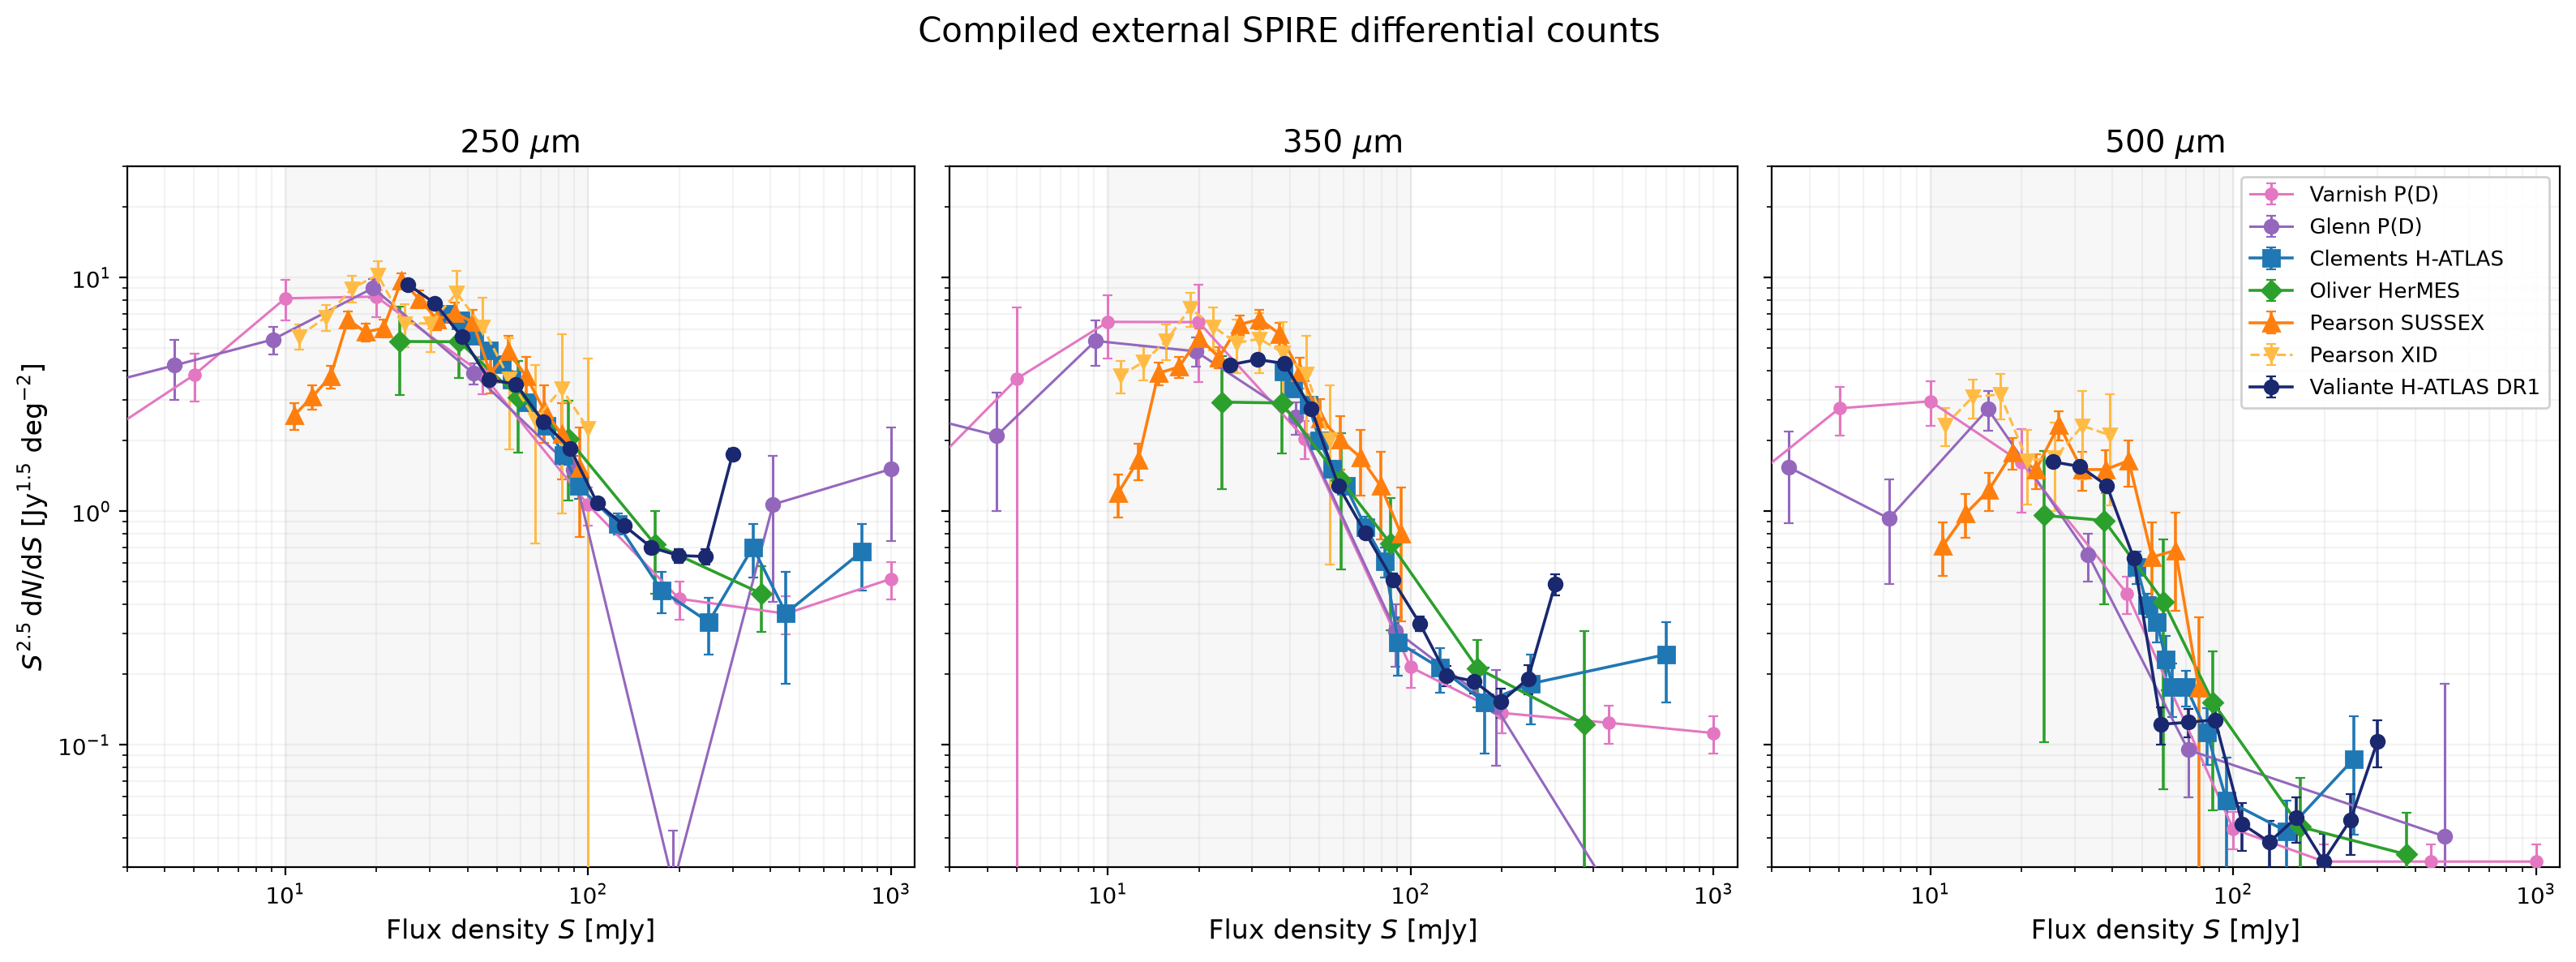
\includegraphics[width=1.2\textwidth]{Figures/compiled_counts_thesis.png}}
\caption{Published Euclidean-normalised differential counts at 250, 350 and
\SI{500}{\um} from the six studies listed in Table~\ref{tab:counts}. The main
 comparison in this work uses the 10--\SI{100}{mJy} range (shaded), where the
 counts are well constrained. The overlap between all three primary survey families is
 strongest above approximately \SI{30}{mJy}.
Bins above \SI{100}{mJy} are shown but treated with caution because the external surveys
contain few objects in their brightest bins, the model covers only the COSMOS area, and
gravitationally lensed sources become increasingly important.}
\label{fig:compiled_counts}
\end{figure}

The source papers use a mixture of steradian- and square-degree-based units. For this
analysis all counts were converted to the common Euclidean-normalised form
$S^{2.5}\,\mathrm{d}N/\mathrm{d}S$, with units of
$\mathrm{Jy}^{1.5}\,\mathrm{deg}^{-2}$. The conversion uses
$1\,\mathrm{sr}=(180/\pi)^2\,\mathrm{deg}^2$. Thus a count reported in
$\mathrm{mJy}^{1.5}\,\mathrm{sr}^{-1}$ is multiplied by
$(10^{-3})^{1.5}(\pi/180)^2$, together with any power-of-ten multiplier printed in the
source table. Published uncertainties are multiplied by the same linear factor. The
three GAMA fields in \citet{Valiante_2016} were combined by weighting their tabulated
counts by their respective areas of 53.43, 53.56 and
\SI{54.56}{\deg\squared}. Upper limits were retained in the data record but excluded
from the numerical score. Converted curves were checked against figures in the source
papers and against overlapping surveys before use.

The P(D) measurements require a different interpretation from the source-extraction
tables. The name refers to the probability distribution of deflections. Here $D$ is the
measured deflection, or flux value, in a map pixel, and P(D) is the probability
distribution of those pixel values. At SPIRE resolution, several faint
galaxies can contribute to one beam and many cannot be detected reliably as separate
sources. A trial differential-count model nevertheless predicts a distribution of pixel
brightnesses once the telescope beam and instrumental noise are included. The P(D)
method varies the count model until this predicted pixel histogram matches the observed
one \citep{Glenn_2010,Varnish_2025}. It can therefore constrain
$\mathrm{d}N/\mathrm{d}S$ below the normal source-detection and confusion limits without
assigning flux to individual galaxies.

The resulting table entries are still number-count constraints and can be plotted in
the same units as the extracted-source counts. They are not, however, a catalogue of
detected objects. Each fitted count knot influences the predicted pixel distribution
over a range of brightnesses, so neighbouring knots can have correlated uncertainties.
The Glenn and Varnish P(D) results are consequently used as overlapping faint-end
checks rather than as independent per-object data or a set of fully independent points
in the headline score.

\subsection{Wang and Jin COSMOS catalogues}
\label{sec:data:catalogues}

Two deblended far-infrared catalogues of the COSMOS field are used for per-object flux
comparisons. \citet{Wang_2024} provides a probabilistic, prior-based deblended catalogue
containing 131,178 rows, of which 128,387 are associated with positive COSMOS2020
identifiers. The remaining 2,791 are radio-only priors. SPIRE flux densities were
extracted using the XID+ framework \citep{Hurley_2017}. \citet{Jin_2018} provides a
super-deblended catalogue of 195,107 sources produced with an independent prior-based
photometry pipeline.

These catalogues were used for a different purpose from the published counts. They provide
individual galaxy flux measurements and uncertainties, which are needed for the
per-object scatter analysis in Section~\ref{sec:results}. They are not
independent sky fields, and their raw entries cannot be compared directly with the
completeness-corrected count tables above. Their agreement with each other instead
provides a control on catalogue extraction. Wang and Jin fluxes for matched sources agree to
0.12--\SI{0.15}{dex}, which is much better than either catalogue's agreement with
\popcosmos{} (0.42--\SI{0.51}{dex}). The large per-object scatter is therefore not
explained by the choice of one of these two deblending pipelines.

\subsection{Data-quality and selection limits}
\label{sec:data:quality}

For per-object comparisons against the Wang catalogue, a signal-to-noise ratio (SNR)
threshold of $\geq 5$ is applied to the Wang flux measurements. This conservative choice
reduces sensitivity to faint-end flux bias and uncertain low-significance measurements.
The injection and recovery tests of \citet{Wang_2024} show that these effects increase
toward fainter fluxes and longer SPIRE wavelengths.
The effect is concentrated in the faint bins. Near \SI{25}{mJy}, the $5\sigma$ cut
retains approximately 95\%, 82\% and 99\% of the corresponding $3\sigma$ samples at
250, 350 and 500~$\upmu$m. By approximately \SI{50}{mJy}, the two selections agree in
all three bands.

The published count tables used as the primary benchmark were already corrected for
completeness and flux boosting by their authors. The main count claims in this work focus on
the approximately 10--\SI{100}{mJy} range, where the corrections are best characterised.
All three primary survey families overlap over approximately 30--\SI{100}{mJy}. Bins above approximately
\SI{100}{mJy} are shown but should be considered with caution, because the COSMOS area
(\SI{1.278}{\deg\squared}) provides few bright sources and lensed objects become more
important at high flux densities.

\section{Methods}
\label{sec:methods}

\subsection{From a rest-frame SED to an observed flux}
\label{sec:methods:flux}

Each galaxy in the \popcosmos{} catalogue has a rest-frame attenuated SED
$L_\nu^\mathrm{rest}(\lambda)$ in units of $L_\odot\,\mathrm{Hz}^{-1}$, stored on a
grid of 5,994 rest-frame wavelengths. To predict the observed SPIRE flux density at an observed wavelength $\lambda_\mathrm{obs}$, the
rest-frame wavelength probed is
\begin{equation}
  \lambda_\mathrm{rest} = \frac{\lambda_\mathrm{obs}}{1+z}\,,
  \label{eq:restlam}
\end{equation}
and the observed flux density is
\begin{equation}
  S_\nu = \frac{(1+z)\,L_\nu^\mathrm{rest}(\lambda_\mathrm{rest})}
               {4\pi\,d_L^2(z)}\,,
  \label{eq:flux}
\end{equation}
where $d_L(z)$ is the luminosity distance. Luminosity distances are computed using the
WMAP9 cosmology ($H_0 = 69.32\;\mathrm{km\,s^{-1}\,Mpc^{-1}}$,
$\Omega_m = 0.2865$) \citep{Hinshaw_2013}, adopted consistently throughout this conversion. The factor
$(1+z)$ converts between rest-frame and observed frequency
intervals (the $K$-correction). $L_\nu^\mathrm{rest}$ is evaluated at
  $\lambda_\mathrm{rest}$ by log--log interpolation on the stored wavelength grid, and the
result is converted to millijanskys.

This calculation samples the SED at each nominal SPIRE wavelength rather than integrating
through the full filter transmission curve. It is a computational approximation applied
consistently to every template. Full bandpass integration could shift individual fluxes
and should be included in future precision or per-object analyses.

As a reproducibility check, the integrated $8$--$\SI{1000}{\um}$ luminosity computed
from the stored SED was compared against the stored \LIR{} value. The median ratio
across a random sample of 500 galaxies is $1.00002$, confirming internal consistency of
the stored normalisation and unit conversion. This is not an independent validation of
the physical accuracy of \LIR{}.

  Later in this work, a median population SED is used. It is constructed by placing
all SEDs in the selected population on the same rest-frame wavelength grid, normalising
each to its \LIR{}, and then taking the median and 16th--84th percentile
  interval. This is different from plotting one galaxy whose \LIR{} happens to fall at the
  population median.

\subsection{Constructing differential number counts}
\label{sec:methods:counts}

For each SPIRE band the predicted fluxes are binned into logarithmically spaced
intervals. The differential count in each bin is
\begin{equation}
  \frac{\mathrm{d}N}{\mathrm{d}S} = \frac{N_\mathrm{bin}}{\Delta S \;\Omega}\,,
\end{equation}
where $N_\mathrm{bin}$ is the number of model galaxies in the bin, $\Delta S$ is the
bin width in janskys, and $\Omega = \SI{1.278}{\deg\squared}$ is the effective catalogue
area. Counts are reported in Euclidean-normalised form,
$S^{2.5}\,\mathrm{d}N/\mathrm{d}S$, with units of
$\mathrm{Jy}^{1.5}\,\mathrm{deg}^{-2}$. For a non-evolving population in Euclidean
space, $\mathrm{d}N/\mathrm{d}S\propto S^{-2.5}$, so this rescaling would produce a
horizontal curve. It does not change the underlying counts. It makes departures from
that simple reference and differences between model and data easier to compare across
the flux range.

\subsection{Alternative far-infrared SED families}
\label{sec:methods:templates}

The main question here is whether the count disagreement improves when using a warmer far-infrared
shape while the learned galaxy population and \LIR{} are held fixed. To answer this, four
  alternative dust prescriptions are substituted in place of the FSPS baseline. In all
  tests, each galaxy's total infrared luminosity is preserved, so the
comparison changes only where in wavelength the energy appears, not how much is emitted.
These substitutions are exploratory. They show the direction of the required correction
but do not identify its underlying physics.

The FSPS baseline is the existing \popcosmos{}/FSPS dust emission shape, used
without modification. The ALESS template is the composite rest-frame
SED of luminous submillimetre galaxies from \citet{daCunha_2015}, renormalised to each
galaxy's \LIR{}. It serves as a warm-shape bracket rather than a universal galaxy
model. FSPS/ALESS hybrids were created by combining the two luminosity-density shapes on a
common rest-frame wavelength grid at 25\%, 50\% and 75\% ALESS contribution, each
renormalised to the original \LIR{}. The modified-blackbody (MBB) grid uses optically
thin, single-temperature shapes, $L_\nu \propto \nu^\beta B_\nu(T)$, with dust
temperatures from 20 to \SI{50}{K} in \SI{5}{K} steps. The emissivity index is fixed at
the assumed value $\beta=1.8$, rather than inferred from the data. Each template is
renormalised over 8--\SI{1000}{\um} to preserve the galaxy's original \LIR{}.
Finally, a Casey-inspired diagnostic replaces the Wien side of the MBB with a continuous
mid-infrared power law, joined where the logarithmic slopes match
\citep{Casey_2012}. This captures the greybody-plus-power-law idea but is not the exact
analytic Casey fitting function. It is treated as a diagnostic parameterisation, not a
complete solution that explains the physics. Figure~\ref{fig:mbb_shapes} shows the modified
blackbody shapes normalised to equal \LIR{}, illustrating how the same total energy
is redistributed across wavelength as dust temperature increases.

% FIGURE: MBB template shapes
\begin{figure}[H]
\centering
\makebox[\textwidth][c]{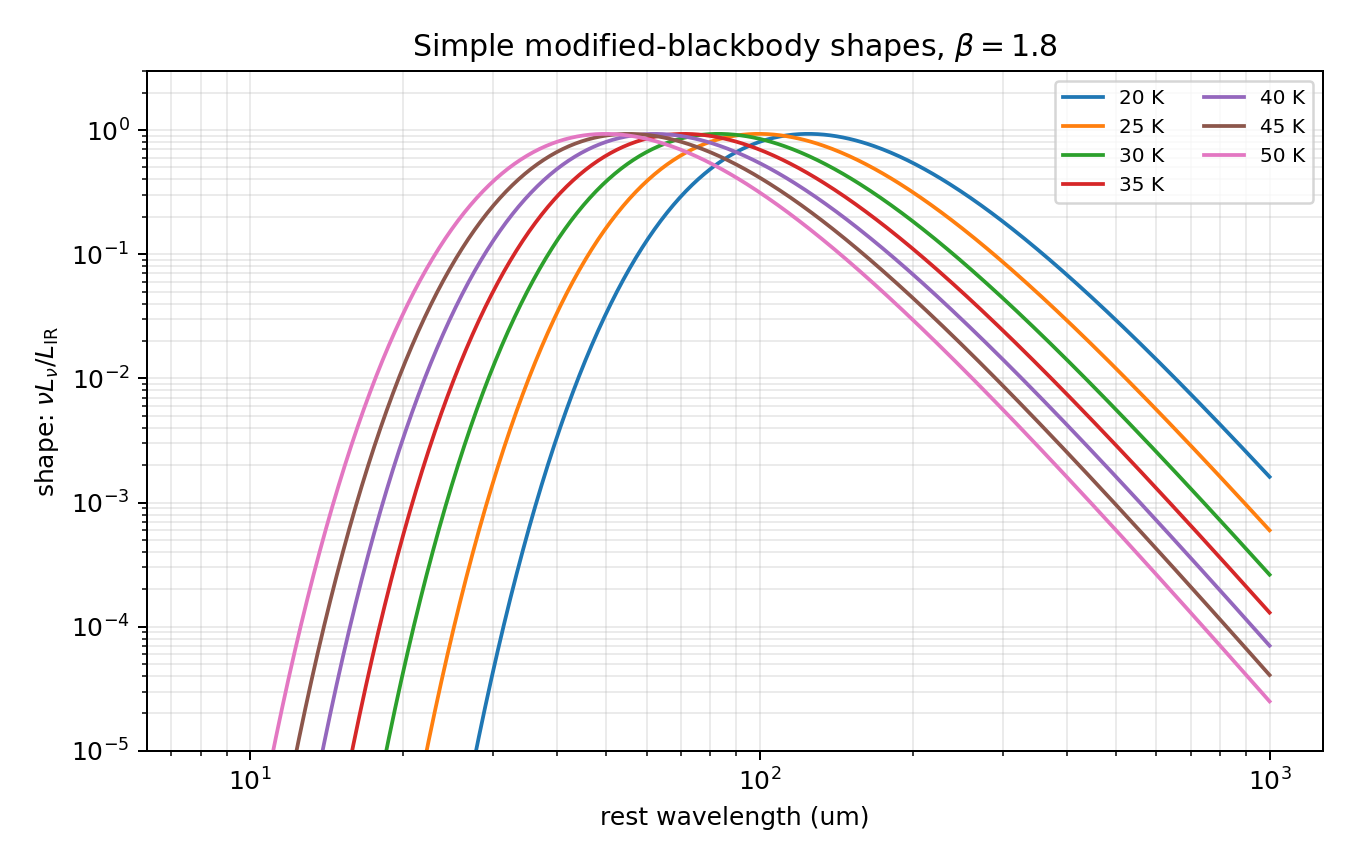
\includegraphics[width=1.15\textwidth]{Figures/popcosmos_mbb_temperature_grid_shapes.png}}
\caption{Modified blackbody dust spectra at temperatures from 20 to \SI{50}{K}
($\beta = 1.8$), each normalised to the same integrated \LIR{}. Warmer dust shifts
the emission peak to shorter wavelengths and reduces the flux at 350 and
\SI{500}{\um} relative to the total. The FSPS baseline peak falls near the 20--25~K
curves.}
\label{fig:mbb_shapes}
\end{figure}

\begin{figure}[H]
\centering
\makebox[\textwidth][c]{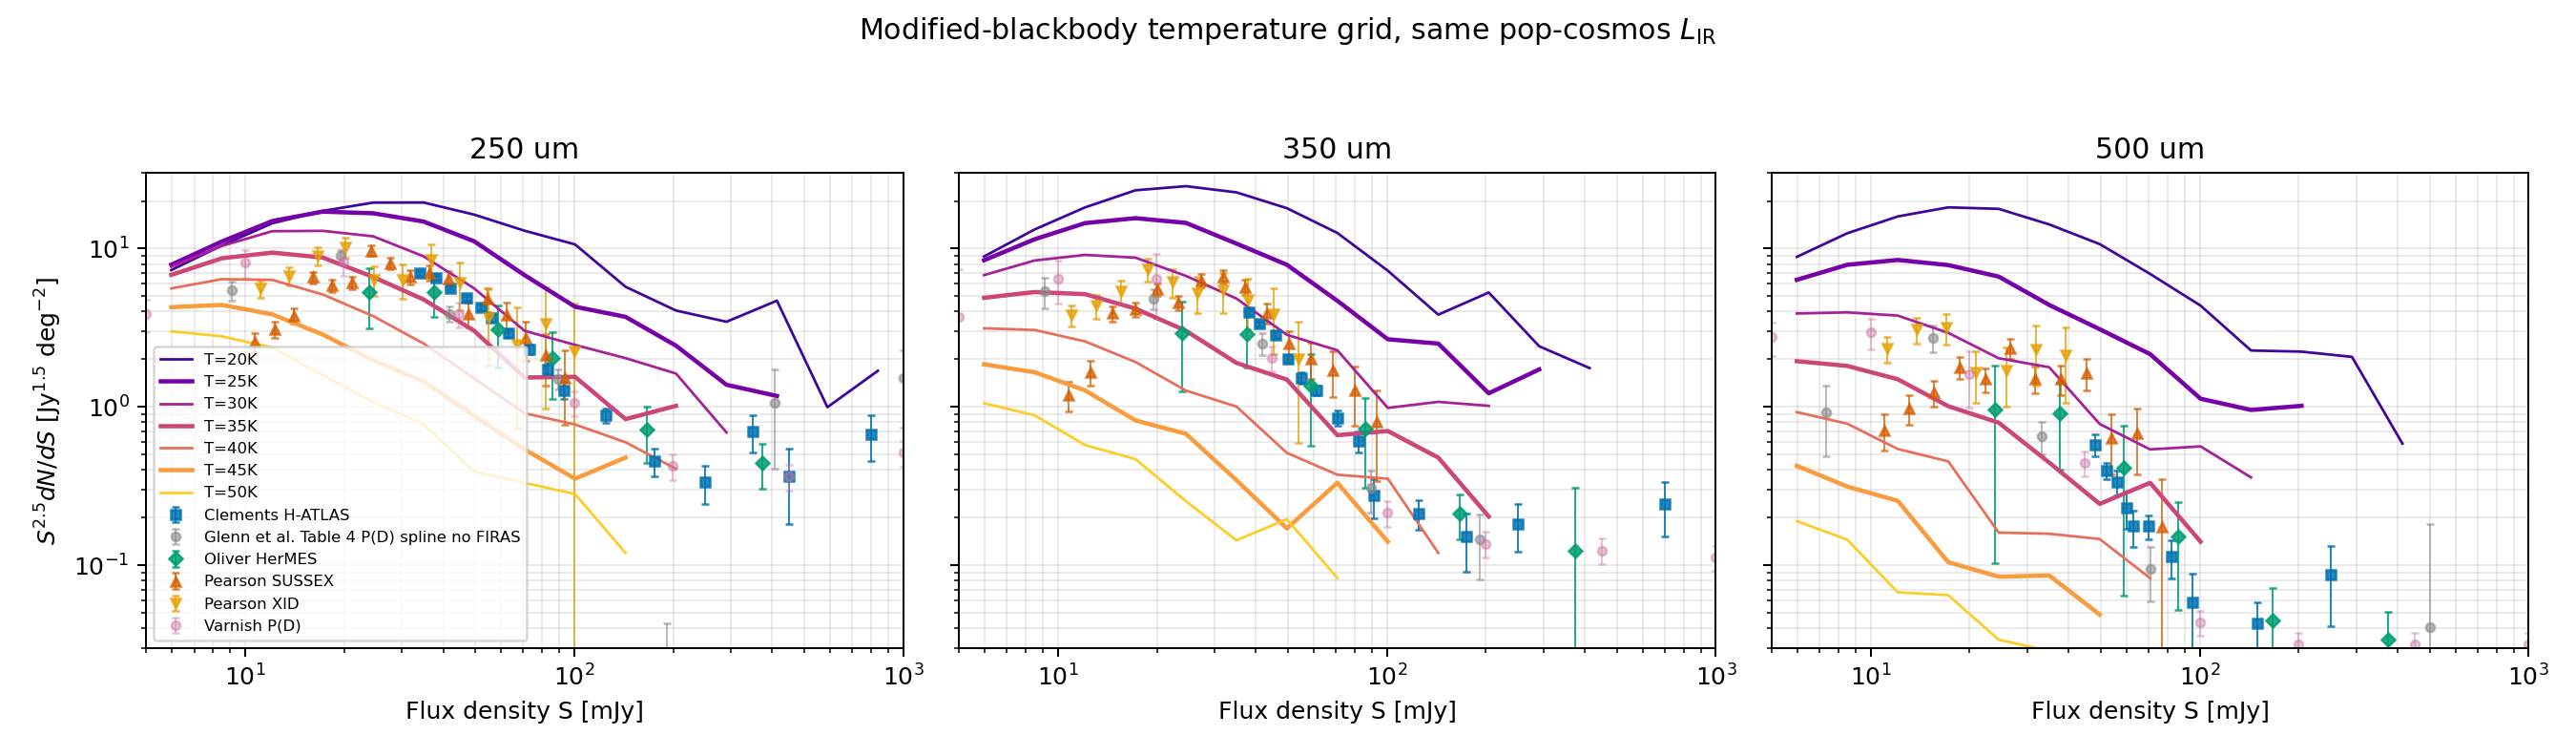
\includegraphics[width=1.15\textwidth]{Figures/popcosmos_mbb_temperature_grid_counts.png}}
\caption{Predicted differential counts for the modified blackbody temperature grid,
  compared against published observations. Each curve uses the same \LIR{} per galaxy,
  and only the dust temperature changes. Intermediate temperatures around 30--\SI{35}{K}
bring the predicted counts closest to the observations, while colder and hotter
extremes both produce worse agreement.}
\label{fig:mbb_counts}
\end{figure}

% FIGURE: analysis pipeline schematic
\begin{figure}[H]
\centering
\makebox[\textwidth][c]{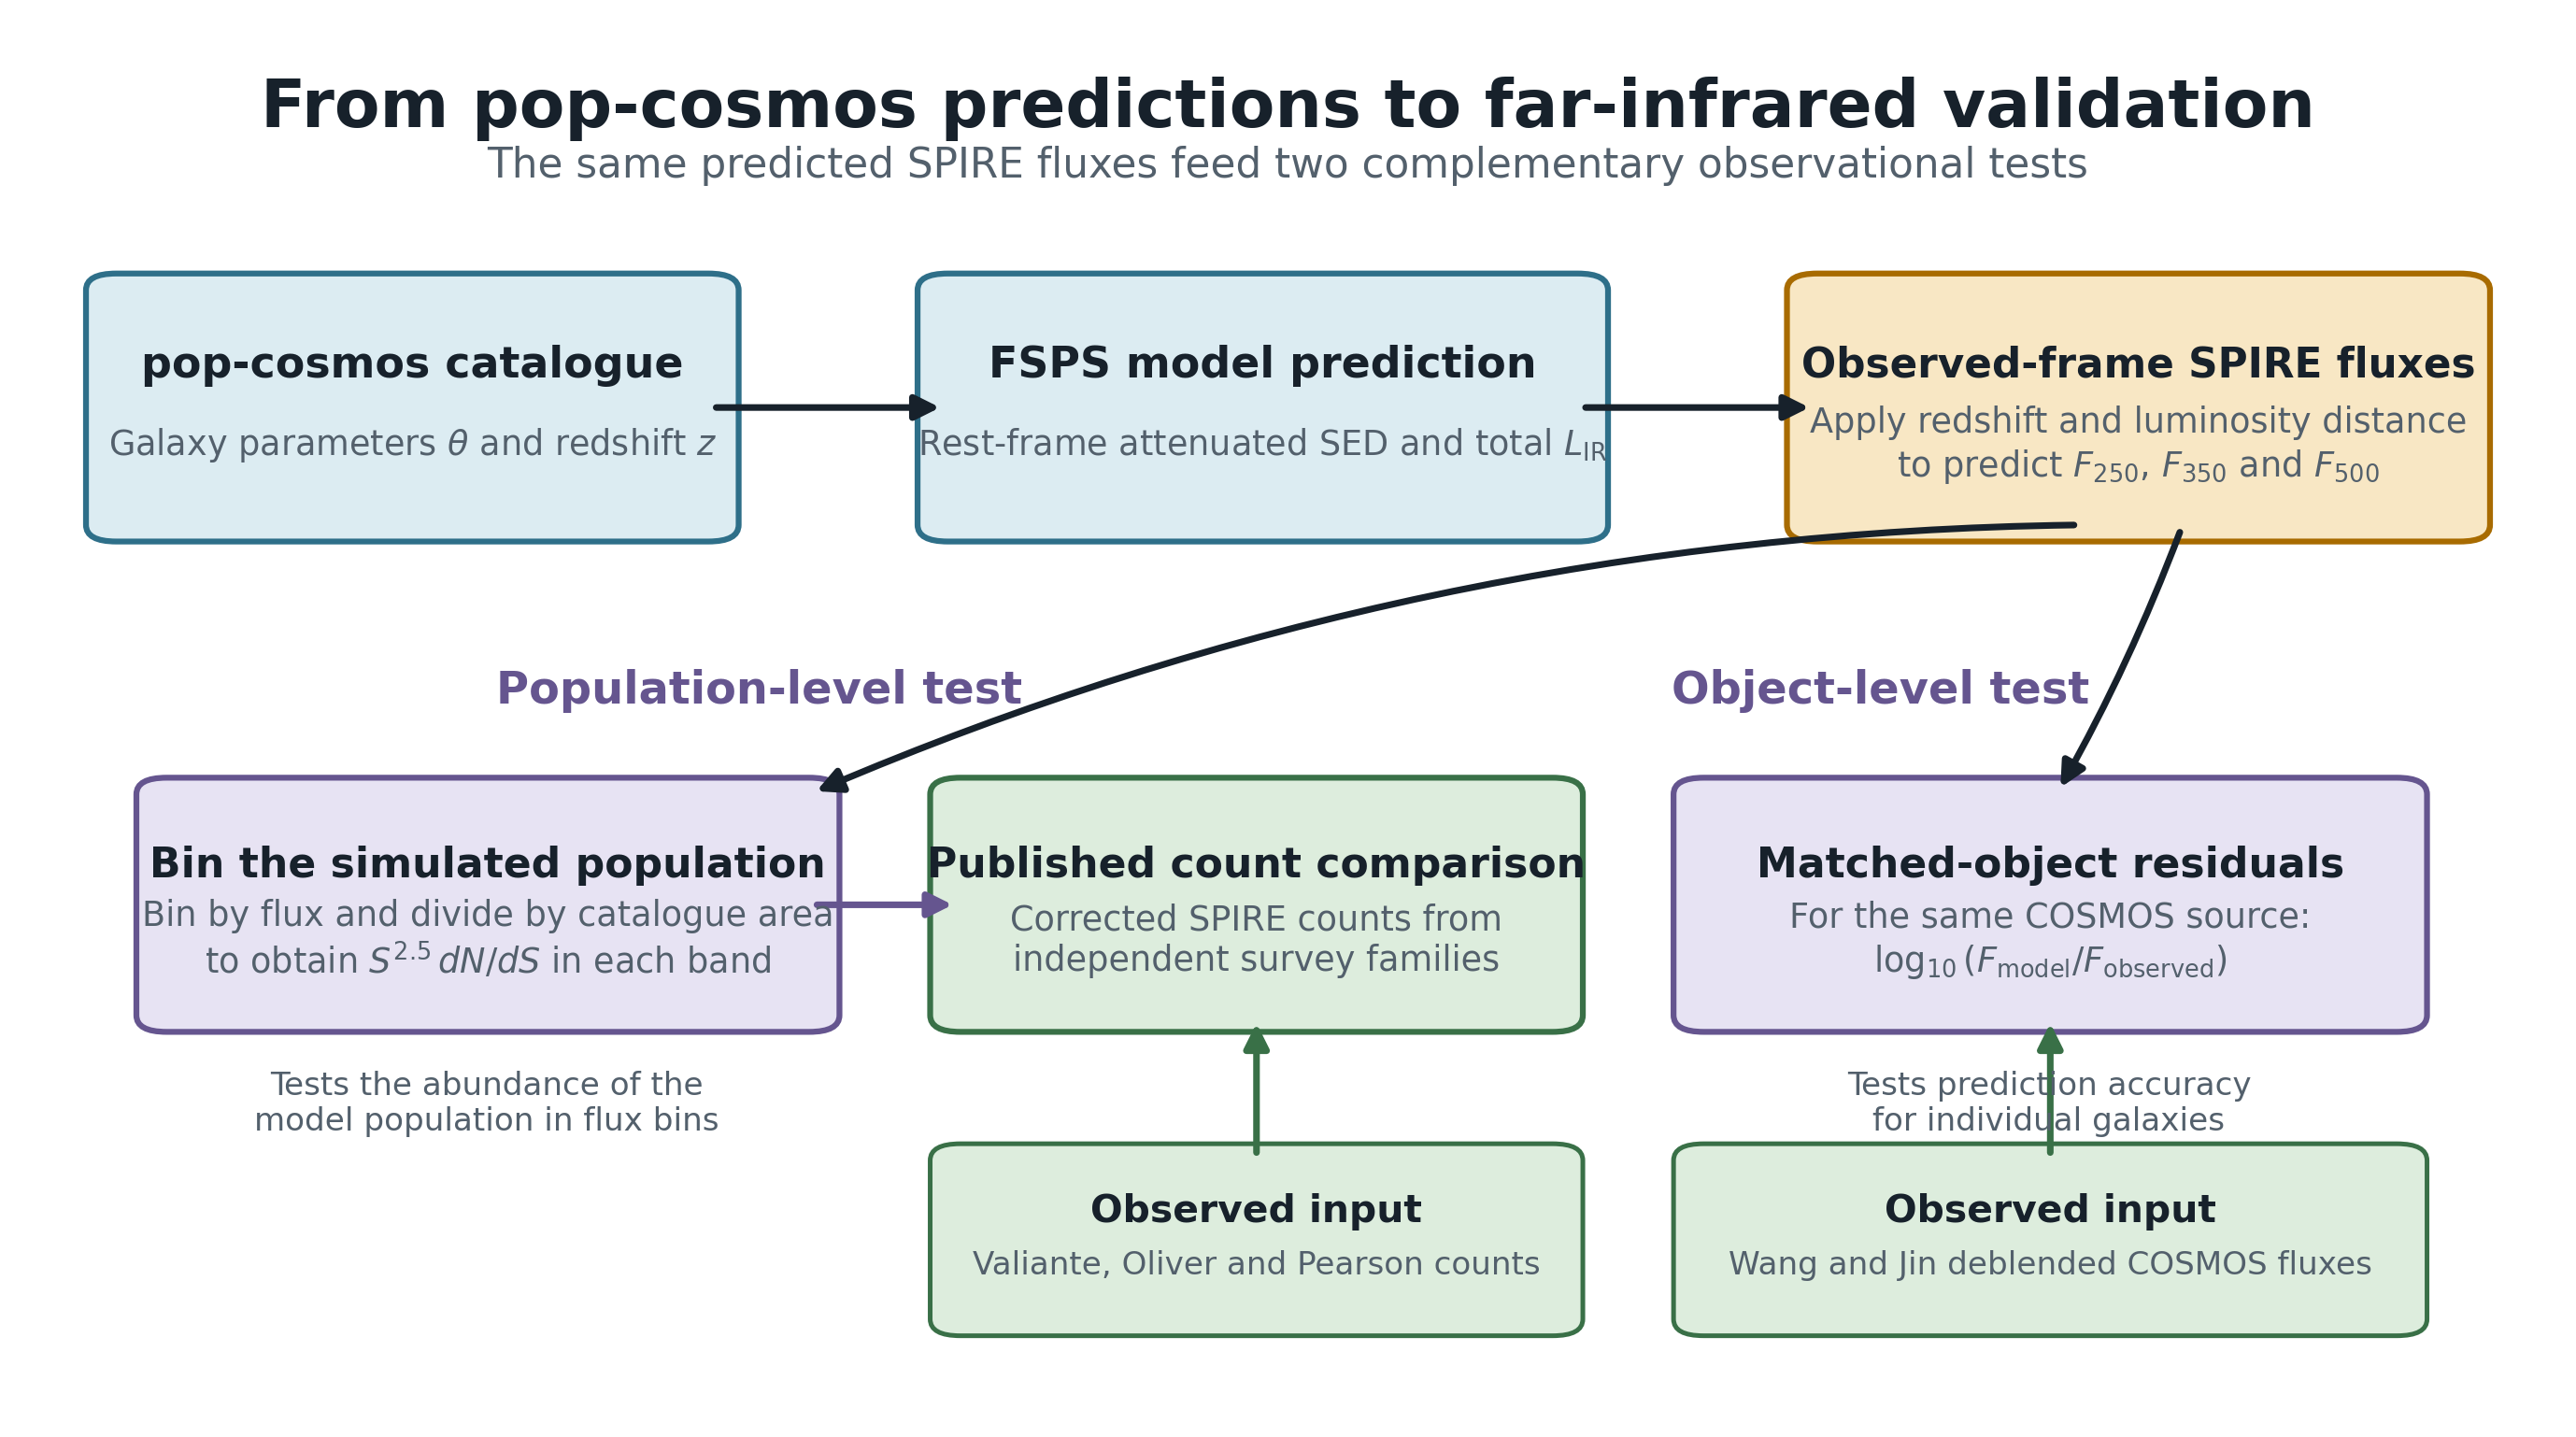
\includegraphics[width=1.15\textwidth]{Figures/popcosmos_fir_validation_pipeline.png}}
\caption{Main work pipeline. \popcosmos{} parameters and redshifts are converted to
rest-frame SEDs via FSPS, then to observed SPIRE fluxes. Differential number counts are compared against published
survey results (left), and per-object fluxes are compared against the Wang and Jin
deblended catalogues (right).}
\label{fig:pipeline}
\end{figure}

\subsection{Count evaluator and error treatment}
\label{sec:methods:evaluator}

Model and published counts are compared using a chi-square evaluator operating in
logarithmic count space. For each published flux bin $i$ with observed
Euclidean-normalised count $C_i^\mathrm{obs}$ and uncertainty $\sigma_i$, the model
count $C_i^\mathrm{mod}$ is obtained by interpolating the model curve to the same flux
value. The log-space residual is
\begin{equation}
  \Delta_i = \log_{10} C_i^\mathrm{mod} - \log_{10} C_i^\mathrm{obs}\,,
\end{equation}
A positive $\Delta_i$ means the model overpredicts. A linear count uncertainty is
converted approximately to log space using
\begin{equation}
  \sigma_{\log,i} = \frac{\sigma_i}{C_i^\mathrm{obs}\ln 10}\,.
\end{equation}
Published uncertainties vary widely in how they are estimated, and some studies quote
very small formal errors that do not reflect the systematic scatter between surveys. The
working uncertainty is therefore
$\widetilde{\sigma}_i=\max(\sigma_{\log,i},0.12\,\mathrm{dex})$. The floor is the
typical scatter measured between independent count families at overlapping fluxes. The
primary statistic is the median $\Delta_i$ across bins. A reduced chi-square-like score,
\begin{equation}
  \chi^2_\nu = \frac{1}{N-k}\sum_i
  \left(\frac{\Delta_i}{\widetilde{\sigma}_i}\right)^2\,,
\end{equation}
is also reported as a rough ranking
measure but is not treated as a formal likelihood, because adjacent flux bins within
the same survey share calibration and completeness corrections and are therefore
correlated. Here $N$ is the number of count bins and $k$ is the number of varied template
parameters.

Each bin is one flux interval from one published table, not an individual galaxy. Only
bins in the 10--\SI{300}{mJy} range with positive, finite model and observed counts enter
the common score.
Because the six studies observe overlapping sky areas
(Section~\ref{sec:data:counts}), treating all of them as independent would overcount
the evidence. For this reason, the chi-square is computed on two sets. The full set uses
174 bins from nine published products across all six studies. The clean set uses only
the 74 bins from Valiante, Oliver
and Pearson, which cover three separate patches of sky and provide the
main test. The model ranking is the same on both sets. As a further check, the
comparison is repeated with a larger error floor and with a block bootstrap that
resamples across the three independent survey families.

\subsection{Object-level residuals and the scatter test}
\label{sec:methods:scatter}

For galaxies matched between the \popcosmos{} predictions and the Wang or Jin
catalogues, per-object residuals are defined as
\begin{equation}
  r = \log_{10}\!\left(\frac{F_\mathrm{model}}{F_\mathrm{observed}}\right).
\end{equation}
Only sources with observed SNR~$\geq 5$ in the relevant band are kept for the primary
matched-object summary. The median
$r$ measures systematic offset, and the 16--84th percentile half-width measures
scatter. Three comparisons are computed (model vs Wang, model vs Jin, Wang vs
Jin) to separate model scatter from deblending scatter. Catalogue flux errors are
propagated into logarithmic units. Their median contribution, $\sigma_\mathrm{noise}$,
is removed in quadrature from the measured residual width,
$\sigma_\mathrm{int}=(\sigma_\mathrm{obs}^2-\sigma_\mathrm{noise}^2)^{1/2}$. This gives
the quoted noise-deconvolved scatter. If the expression is negative it is set to zero.

The scatter has a direct consequence for the counts. With a decreasing source
distribution, symmetric per-object scatter has an asymmetric effect on number
counts, because more faint sources are scattered upward than bright sources are
scattered downward. To quantify this, model galaxies are selected above a predicted
flux cut, such as \SI{20}{mJy}, and the number also observed above the same cut is
measured. This separates model-bright sources confirmed as bright in the data from
those placed above the model threshold by the broad residual distribution. The
mechanism is mathematically analogous to
Eddington bias, although here the scatter is between model predictions and measured
fluxes rather than measurement noise alone. The decomposition uses the wider
$\mathrm{SNR}\geq3$ matched sample to retain enough objects at 350 and
\SI{500}{\um}; its sensitivity to stricter cuts is reported separately.

\subsection{Physical diagnostics}
\label{sec:methods:diagnostics}
Three further diagnostics ask where the model goes wrong beyond the overall count
mismatch. The first uses the observed pattern in which more luminous galaxies have
warmer dust that peaks at shorter wavelengths. \citet{Drew_2022} calibrated this
relationship over $0<z<2$ and found no measurable redshift evolution within that range.
For each low-AGN ($f_\mathrm{AGN}<0.1$) \popcosmos{} galaxy, the rest-frame FIR peak
wavelength is measured and plotted against infrared luminosity. The quantitative
comparison with the observed relation is restricted to $z\leq2$. This tests whether the
model dust is too cold, too uniform, or both.

The second test asks which galaxies are responsible for the count excess. Model galaxies
are split into redshift bins, and one bin is removed at a time. The bin whose removal
reduces the excess by the largest amount contributes most strongly. This matters because
the same observed SPIRE band samples different rest-frame wavelengths at different
redshifts, so the cold-dust problem does not necessarily affect all epochs equally.

A third diagnostic separates ordinary FIR peaks from the unusual short-wavelength
branch visible in some generated SEDs. A reproducible random sample of 8,000 galaxies
is classified as hot-peaking when $\lambda_\mathrm{peak}<\SI{40}{\um}$ and cold-peaking
when $\lambda_\mathrm{peak}>\SI{100}{\um}$. The hot fraction is then measured in bins
of $f_\mathrm{AGN}$. To test whether an average SED represents this mixture, galaxies
are also divided into five \LIR{} bins, normalised by their individual \LIR{} values,
and combined on the common rest-frame grid using both a mean and a median. These stacked
peaks are compared with the distribution of individual peak wavelengths.

\section{Results}
\label{sec:results}

\subsection{Control test where the model is constrained}
\label{sec:results:control}

Before testing the far-infrared predictions, it is useful to confirm that \popcosmos{}
works well over the wavelengths used to constrain it. Predicted and observed IRAC
magnitudes were compared for all galaxies with coverage in each channel.
At Ch1 (\SI{3.6}{\um}), 423,272 galaxies had a median residual of $+0.020$ mag with
a median absolute deviation (MAD) of 0.084 mag. At Ch2 (\SI{4.5}{\um}), 414,272
galaxies yield $-0.012$ mag (MAD 0.041 mag). These residuals are small enough to
  support the consistency of the catalogue, SED products and comparison code over this
  wavelength range. Ch3 and Ch4 have lower coverage and are therefore weaker tests.

% FIGURE: IRAC control test
\begin{figure}[H]
\centering
\makebox[\textwidth][c]{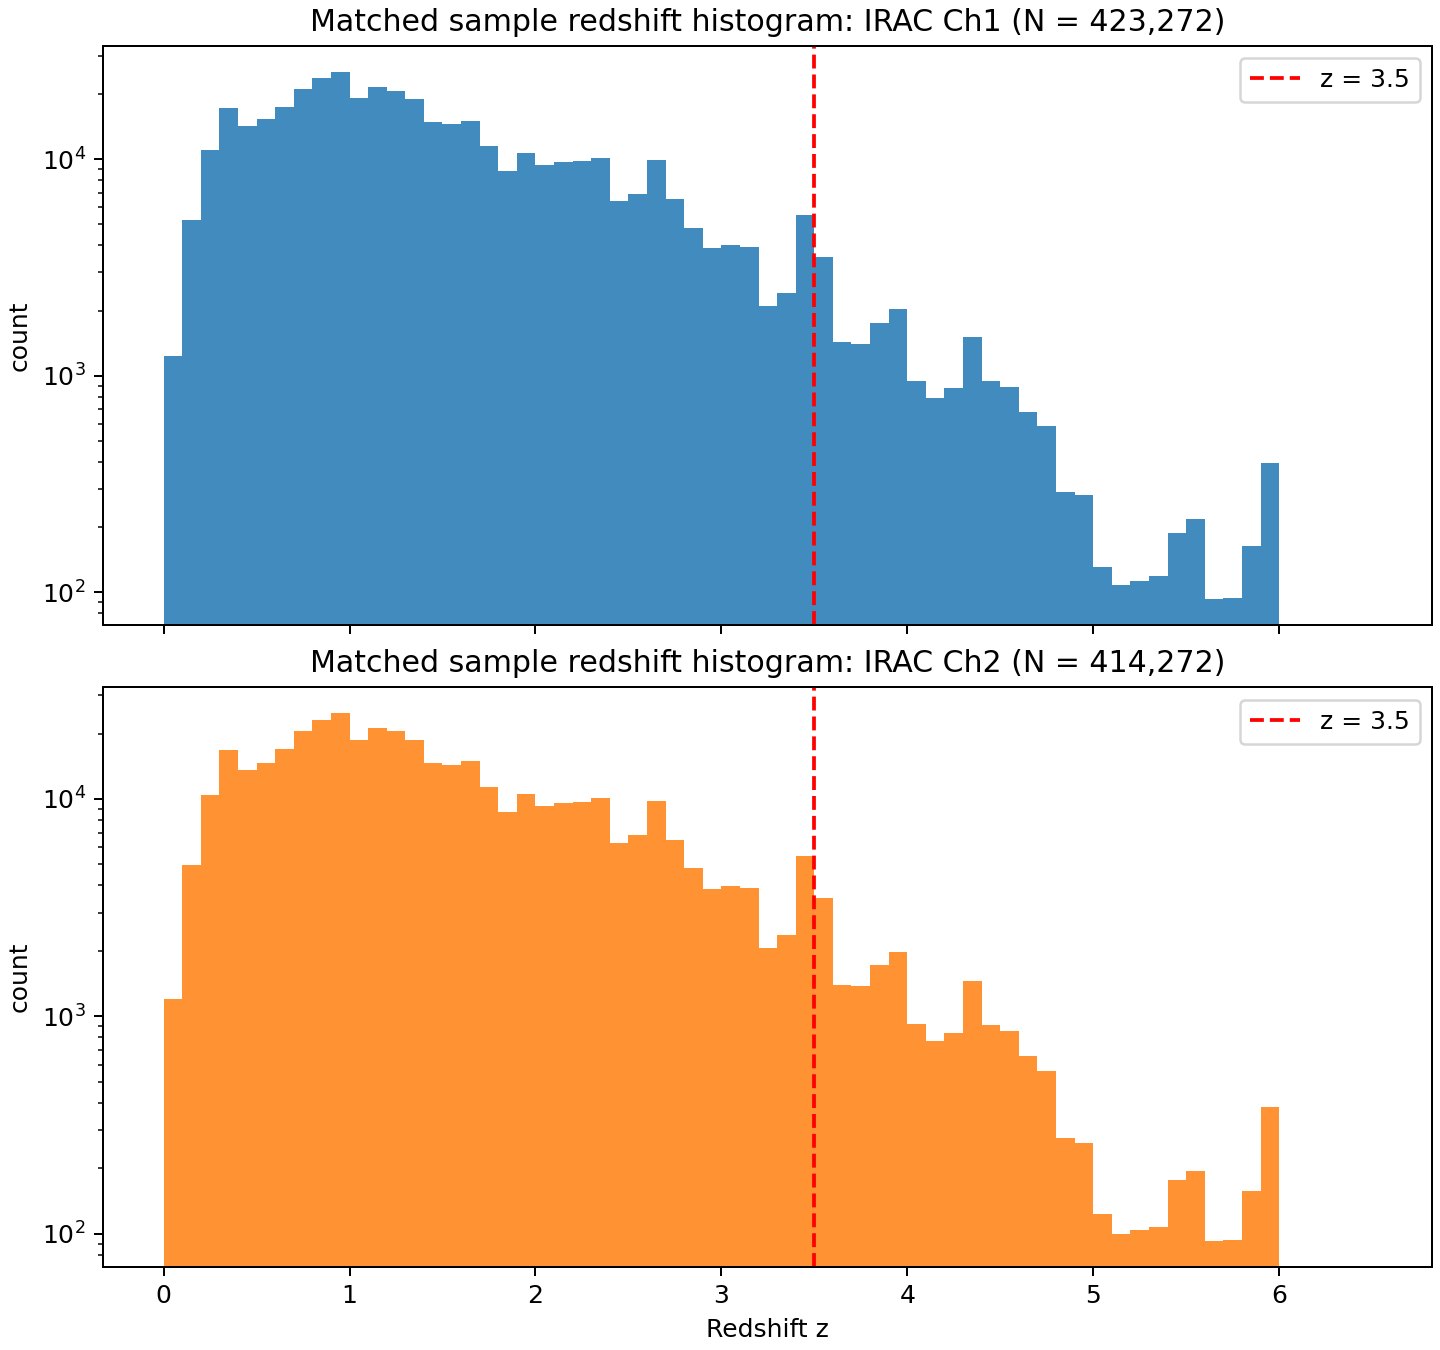
\includegraphics[width=1.15\textwidth]{Figures/popcosmos_irac_redshift_histograms.png}}
\caption{Predicted vs observed IRAC Ch1 and Ch2 magnitudes as a function of redshift.
The model reproduces the near-infrared photometry to within a few hundredths of a
  magnitude across the full redshift range. This supports the interpretation that the
  far-infrared discrepancy reported below is wavelength-dependent rather than a general
  catalogue offset.}
\label{fig:irac_control}
\end{figure}

\subsection{Published far-infrared number counts}
\label{sec:results:counts}

% FIGURE: headline count overlay
\begin{figure}[H]
\centering
\makebox[\textwidth][c]{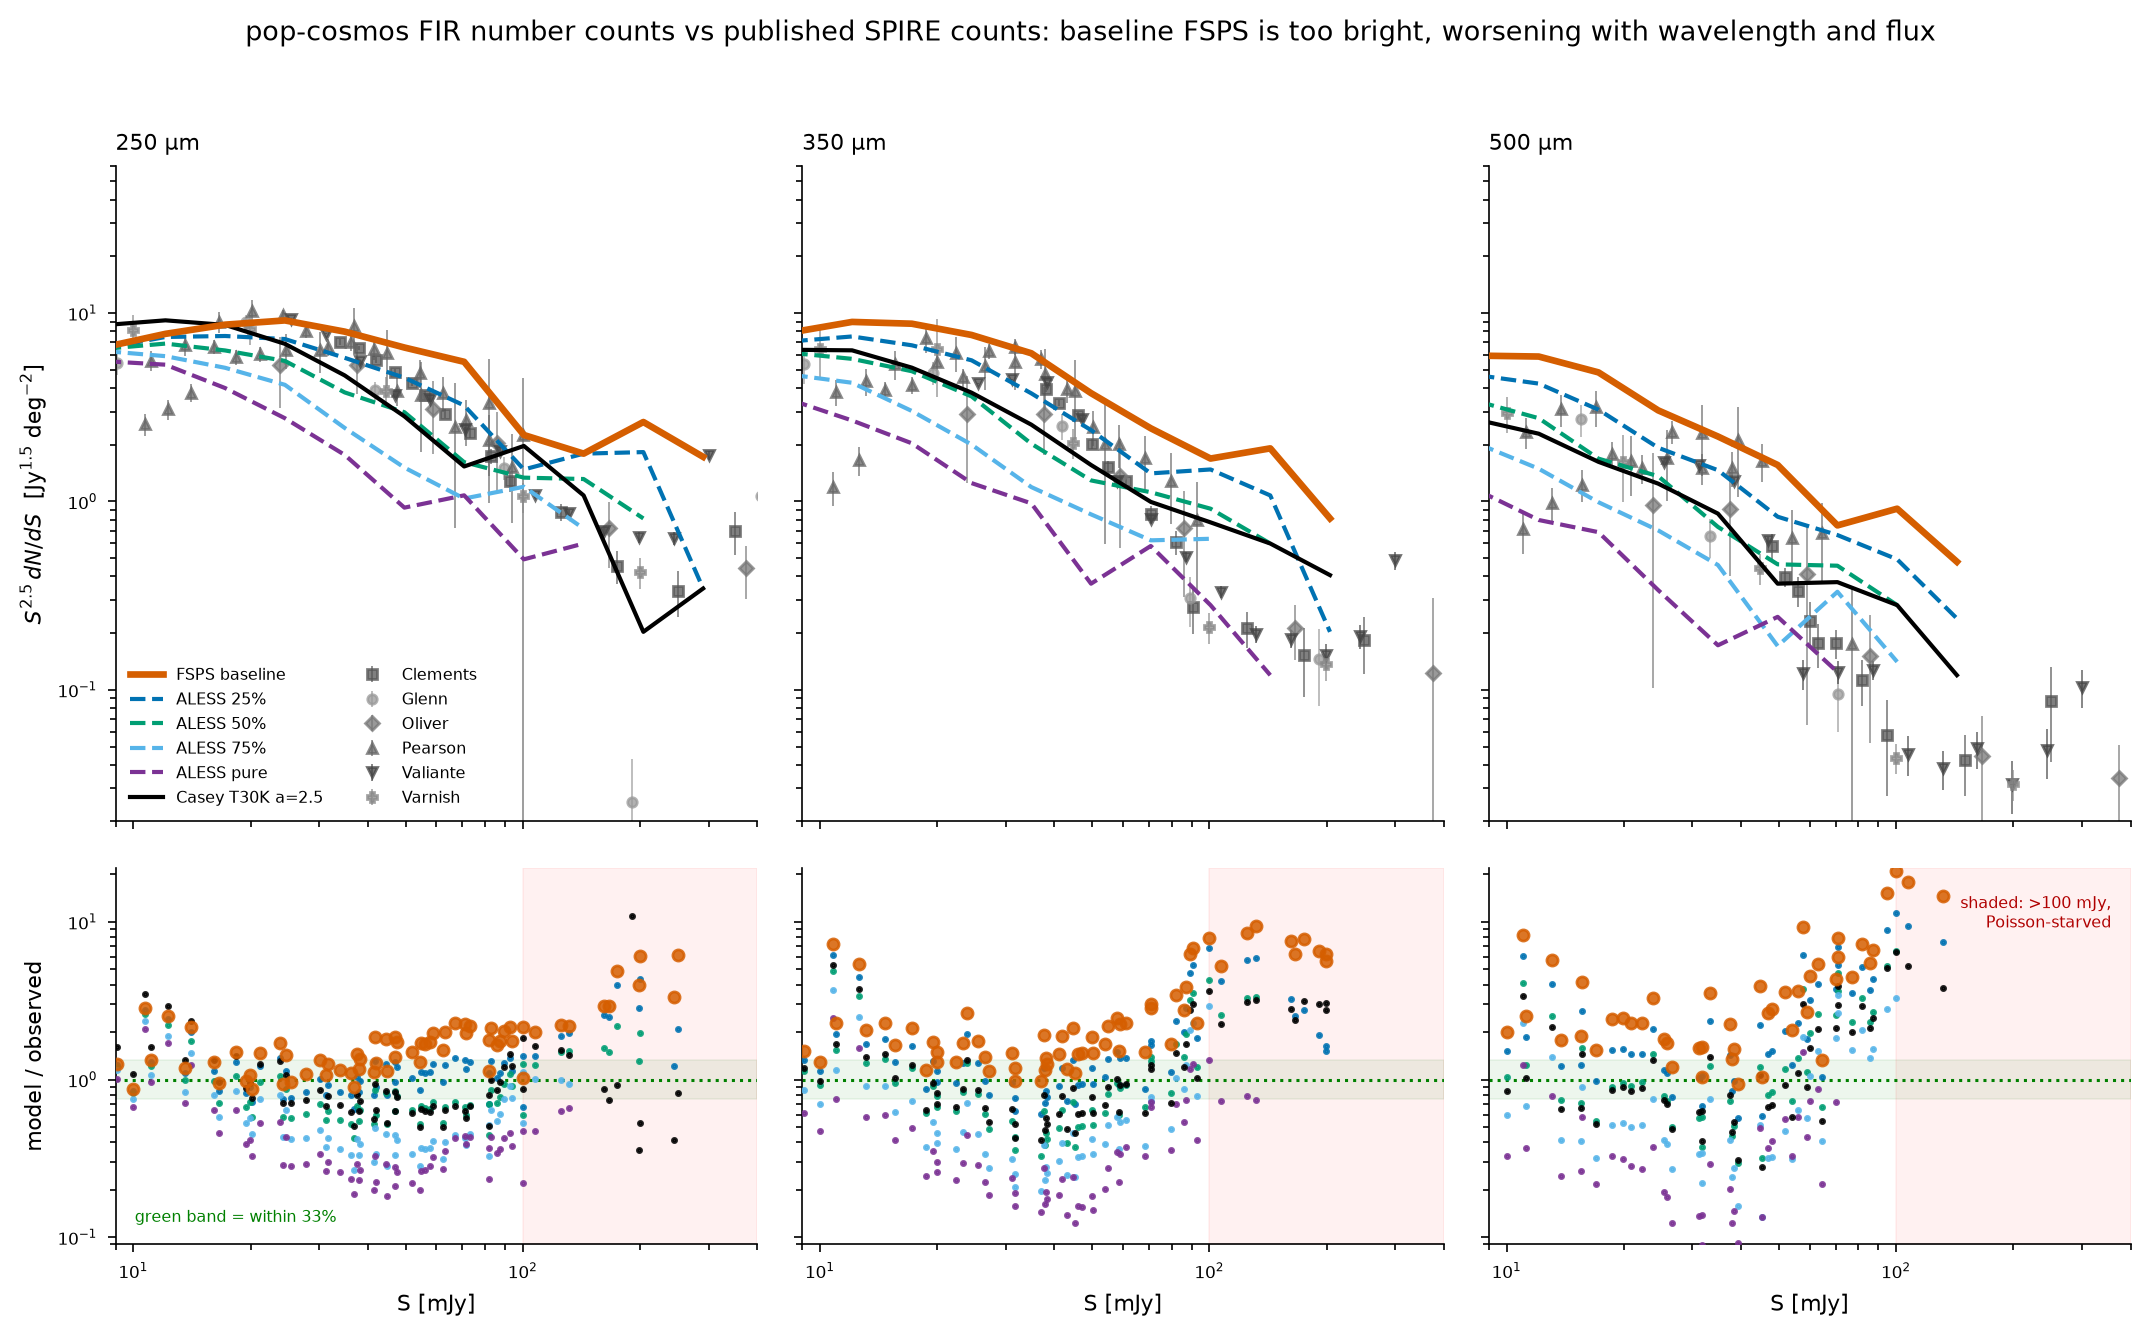
\includegraphics[width=1.15\textwidth]{Figures/popcosmos_count_overlay_thesis.png}}
\caption{Euclidean-normalised differential counts at 250, 350 and \SI{500}{\um}.
Coloured points are the published observations shown in Table~\ref{tab:counts}. The solid line is
  the baseline \popcosmos{}/FSPS prediction. The model overpredicts in all three bands,
with the excess increasing at longer wavelengths. Dashed and dotted lines show the
alternative dust prescriptions with a fixed \LIR{} as discussed above (Section~\ref{sec:results:templates}).}
\label{fig:count_overlay}
\end{figure}

The baseline model overpredicts the counts in all three bands. In the well-constrained
30--\SI{100}{mJy} range, the excess is approximately $1.7\times$ at both 250 and
\SI{350}{\um}, increasing to approximately $3.6\times$ at \SI{500}{\um}. Expressed as
median log residuals across the full scorecard, the offsets are $+0.25$, $+0.41$ and
$+\SI{0.55}{dex}$ at 250, 350 and \SI{500}{\um}, respectively.
  These two summaries use different flux ranges and pooling methods. The 30--100 mJy
factors come from the regime where all three primary survey families overlap, whereas the
  median residuals span the full 10--300 mJy range. Both measures agree that the excess
  has the same sign in each independent survey-family benchmark and rises with wavelength.
  In every band, the baseline residual is larger than the empirical survey-to-survey
  scatter used in the evaluator.

Table~\ref{tab:fsps_regimes} resolves this result by flux range. The baseline is already
high at 10--\SI{30}{mJy}, especially at 350 and \SI{500}{\um}. It remains high over
30--\SI{100}{mJy}, where the survey overlap is strongest, and then rises sharply above
\SI{100}{mJy}. The final regime contains relatively few published bins and is affected
by lensing and small-number statistics, so its large factors are evidence of a bright-end
failure but are not used as the primary quantitative claim.

\begin{table}[H]
\centering
\caption{Baseline FSPS residuals separated by SPIRE band and flux regime. $N$ is the
number of published count bins entering each median. Positive residuals indicate too
many model sources.}
\label{tab:fsps_regimes}
\footnotesize
\begin{tabular}{@{}rrrrr@{}}
\toprule
Band & Flux range & $N$ & Median residual & Model/data factor \\
($\upmu$m) & (mJy) & & (dex) & \\
\midrule
250 & 10--30  & 18 & $+0.093$ & 1.24 \\
250 & 30--100 & 38 & $+0.223$ & 1.67 \\
250 & 100--300 & 13 & $+0.467$ & 2.93 \\
350 & 10--30  & 18 & $+0.236$ & 1.72 \\
350 & 30--100 & 33 & $+0.227$ & 1.69 \\
350 & 100--300 & 13 & $+0.798$ & 6.28 \\
500 & 10--30  & 16 & $+0.359$ & 2.29 \\
500 & 30--100 & 28 & $+0.552$ & 3.57 \\
500 & 100--300 & 11 & $+1.163$ & 14.57 \\
\bottomrule
\end{tabular}
\end{table}

\subsection{The baseline SED is too cold and too uniform}
\label{sec:results:cold}

  The count excess at long wavelengths suggests that the model places too much emission
  on the long-wavelength side of its far-infrared peak. To test this independently of the template experiment, the
rest-frame far-infrared peak wavelength $\lambda_\mathrm{peak}$ of each low-AGN
($f_\mathrm{AGN} < 0.1$) model galaxy was measured and compared against infrared
luminosity.

% FIGURE: Drew & Casey peak relation
\begin{figure}[H]
\centering
\makebox[\textwidth][c]{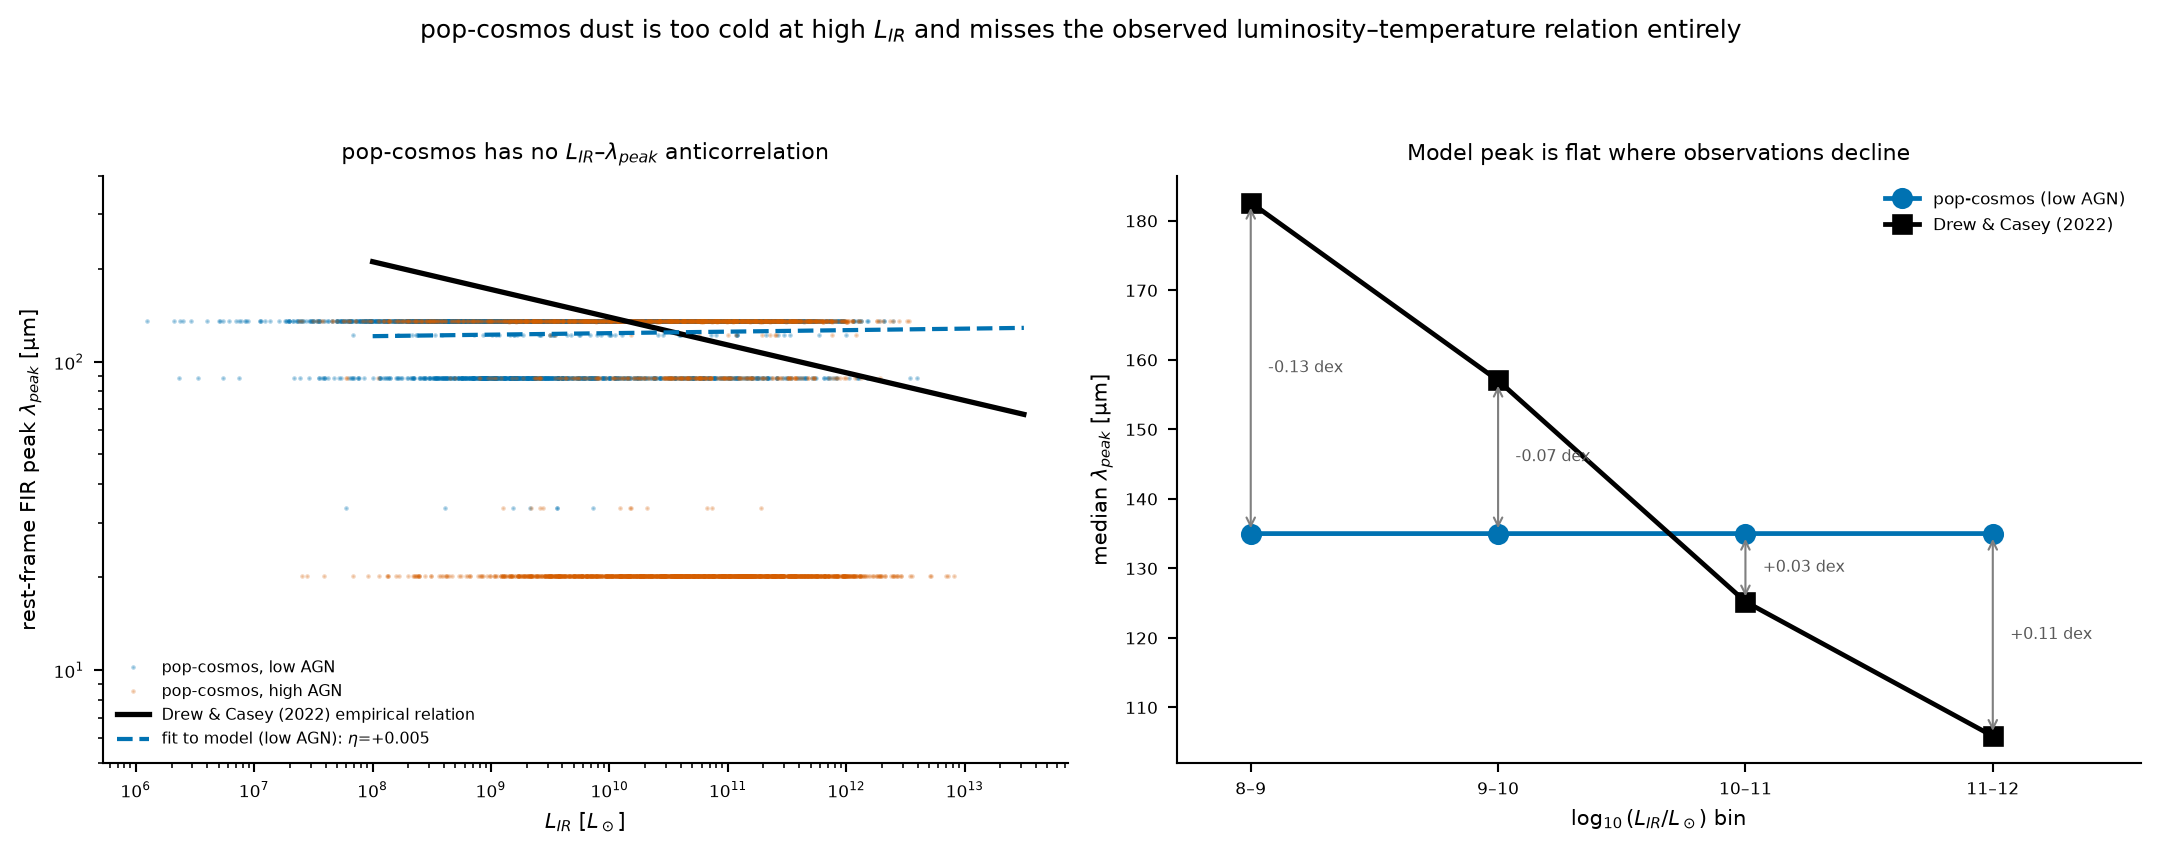
\includegraphics[width=\textwidth]{Figures/drew_casey_peak_relation.png}}
\caption{Rest-frame far-infrared peak wavelength vs infrared luminosity for
\popcosmos{} galaxies, separated by the model AGN parameter, and the observed relation
from \citet{Drew_2022} (red line). The observed relation has slope
$\eta=-0.09\pm0.01$, so more luminous galaxies have warmer, shorter-peaking dust. The
dashed low-AGN fit to the full exploratory model sample is nearly flat
($\eta=+0.005$). Restricting the comparison to the observed calibration range
$z\leq2$ gives the same conclusion, with $\eta=+0.004$ and a fitted peak of
approximately \SI{126}{\um}, compared with \SI{92}{\um} at
$L_\mathrm{IR}=10^{12}\,L_\odot$.}
\label{fig:drew_casey}
\end{figure}

\citet{Drew_2022} calibrated a quantitative relation over $0<z<2$ and found no
measurable redshift evolution within that interval. The relation has
$\lambda_\mathrm{peak} \propto L_\mathrm{IR}^{-0.09}$, with
$\lambda_\mathrm{peak} \approx \SI{92}{\um}$ at
$L_\mathrm{IR} = 10^{12}\,L_\odot$. Restricting the low-AGN model sample to
$z\leq2$ leaves 2,805 galaxies. Its fitted relation peaks near \SI{126}{\um} at the
same luminosity and has an essentially flat slope, $\eta=+0.004$. The unrestricted
  exploratory sample gives a similar slope, $\eta=+0.005$. The model therefore has two
mismatches with the benchmark. Its fitted normalisation is offset to colder dust, and
its peak wavelength shows no meaningful luminosity trend. The model also has an unusually narrow range of peak
wavelengths. The missing luminosity dependence means the bright, luminous population
remains too cold at the wavelengths where the SPIRE counts are most sensitive.

The low-AGN selection is important because the full catalogue contains a second,
short-wavelength peak population. That branch is examined separately below rather than
being allowed to alter the star-forming dust comparison.

\subsection{A separate AGN-associated hot SED branch}
\label{sec:results:agn}

The distribution of individual SED peaks is bimodal rather than a single broad dust
temperature sequence. In a random sample of 8,000 model galaxies, 2,484 (31.1\%) peak
below \SI{40}{\um}, with a median peak near \SI{14}{\um}. A further 4,403 (55.0\%) peak
beyond \SI{100}{\um}, with a median of \SI{135.5}{\um}. The short-wavelength group is
strongly associated with the model AGN parameter. Only 0.3--1.0\% of galaxies with
$f_\mathrm{AGN}<0.1$ peak below \SI{40}{\um}, compared with 13\% at
$0.1\leq f_\mathrm{AGN}<0.3$, 67\% at $0.3\leq f_\mathrm{AGN}<1$, and 100\% at
$f_\mathrm{AGN}\geq1$. Overall, 93.9\%
of hot-peaking galaxies have $f_\mathrm{AGN}>0.3$. These values support an AGN/torus
origin for the unusual mid-infrared bump rather than interpreting it as the peak of
ordinary star-forming dust.

\begin{figure}[H]
\centering
\makebox[\textwidth][c]{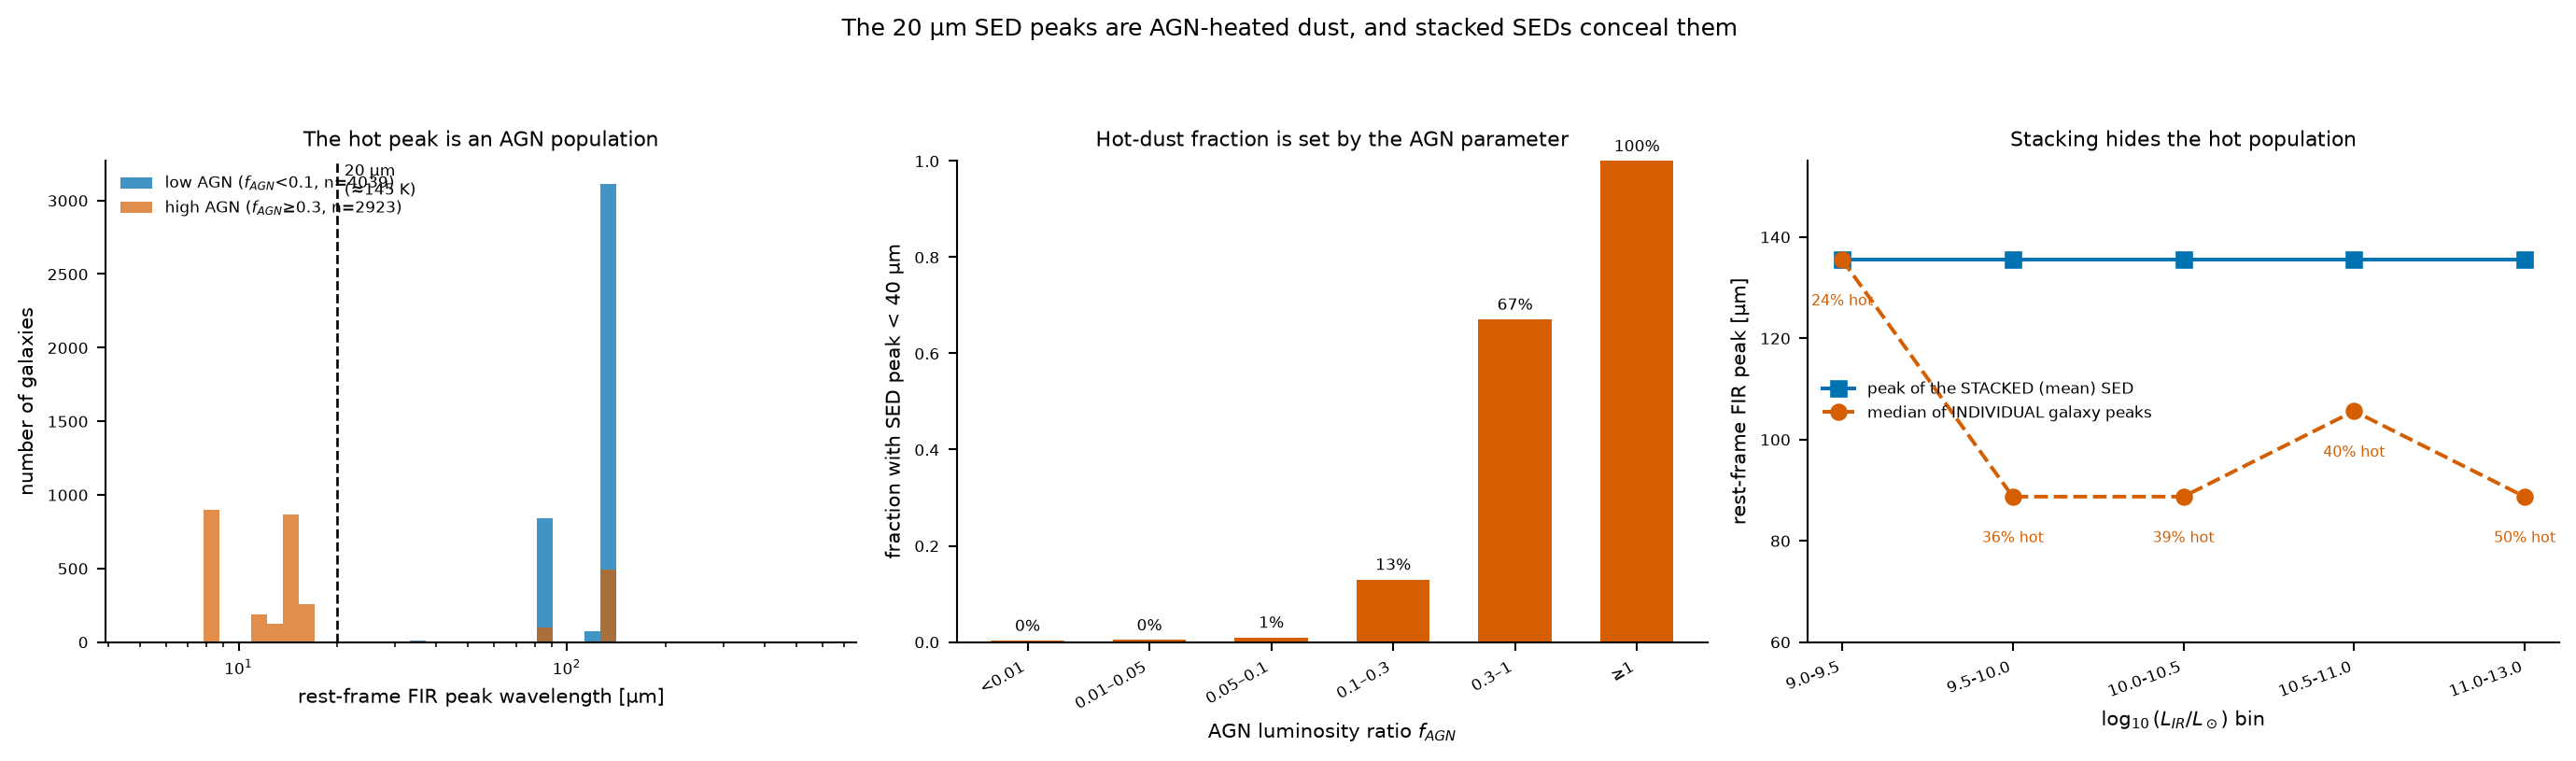
\includegraphics[width=1.15\textwidth]{Figures/agn_hot_dust_diagnosis.png}}
\caption{Diagnosis of the short-wavelength SED branch. Left: individual peak
wavelengths separate into a hot branch near \SI{14}{\um} and a cold branch near
\SI{136}{\um}; the hot branch is dominated by high-$f_\mathrm{AGN}$ objects. Centre:
the fraction peaking below \SI{40}{\um} rises steeply with the model AGN luminosity
ratio. Right: the peak of an \LIR{}-normalised stacked SED remains near
\SI{136}{\um} in every luminosity bin even when 24--50\% of the individual galaxies in
that bin are hot-peaking. A stack can therefore hide the second population.}
\label{fig:agn_hot_branch}
\end{figure}

This diagnostic also tests how the population SED should be summarised. Taking the mean
or median luminosity-normalised SED gives a peak at \SI{135.5}{\um} in every \LIR{} bin
examined,
even in the highest-luminosity bin where half of the individual galaxies peak below
\SI{40}{\um}. The cold component dominates the stacked energy distribution, so one
stack does not represent the diversity of individual shapes. The report therefore uses
the distribution of individual peak wavelengths for the AGN diagnostic and the low-AGN
sample for the star-forming dust relation.

This is evidence about the internal behaviour of the fitted model, not a measurement of
the true AGN fraction in COSMOS. The $f_\mathrm{AGN}$ parameter is not an external AGN
classification, and its prior is bimodal \citep{Thorp_2025_insights}. Because the SEDs
were generated from posterior-median parameters, a median can fall on one branch or
conceal posterior mass on the other. Propagating full posterior samples would be needed
to establish how much of the inferred hot population is constrained by the photometry.

The effect also appears in the predicted photometry. Comparing low- and high-AGN
galaxies within the same \LIR{} and redshift bins gives a median high/low predicted
\SI{250}{\um} flux ratio between 0.41 and 0.60. The typical value is approximately
0.53, so the model AGN component redirects a substantial fraction of fixed \LIR{} away
from the cool-dust wavelength range. This can contribute to faint individual FIR
predictions for AGN-dominated objects, but it cannot explain the population count
excess, which remains present in the low-AGN cold branch.

\subsection{Controlled template experiments}
\label{sec:results:templates}

To confirm that the count excess responds to a warmer far-infrared shape, the
alternative dust models described in Section~\ref{sec:methods:templates} were
substituted with a fixed \LIR{}. The resulting count curves are included in
Figure~\ref{fig:count_overlay} as dashed or dotted lines.

Warmer templates reduce the excess in the expected direction. The best-scoring
alternatives in the unified 174-point comparison are Casey $T = \SI{30}{K}$,
$\alpha = 2.5$ (median residual $-\SI{0.06}{dex}$) and Casey $T = \SI{30}{K}$,
$\alpha = 3.0$ ($+\SI{0.03}{dex}$). The MBB at \SI{35}{K} ($-\SI{0.12}{dex}$) and the
50\% ALESS/FSPS hybrid ($-\SI{0.08}{dex}$) also perform well. All four have median
offsets within the \SI{0.12}{dex} inter-survey scale. This does not mean that every flux
bin is fitted. In the cleaner 74-point three-family
evaluation, the ranking is similar, with Casey $T = \SI{30}{K}$, $\alpha = 3.0$ scoring
best (median $+\SI{0.01}{dex}$).

The improvement is consistent across the count checks but is not diagnostic of one
physical model. Several template families score
similarly within inter-survey scatter, so the counts support a warmer and more
luminosity-dependent direction but do not select a dust prescription. The FSPS
baseline remains positive in the survey-family block bootstrap (median
  $+\SI{0.29}{dex}$, 95\% bootstrap interval $[+0.16,+0.52]$), while the best-scoring
alternatives hover around zero. This interval is a robustness summary instead of a formal
95\% exclusion because only three independent survey families are available.

\subsection{Per-object scatter is a second problem}
\label{sec:results:scatter}

A separate issue is seen when comparing individual galaxies rather than population
counts.

% FIGURE: scatter mechanism
\begin{figure}[H]
\centering
\makebox[\textwidth][c]{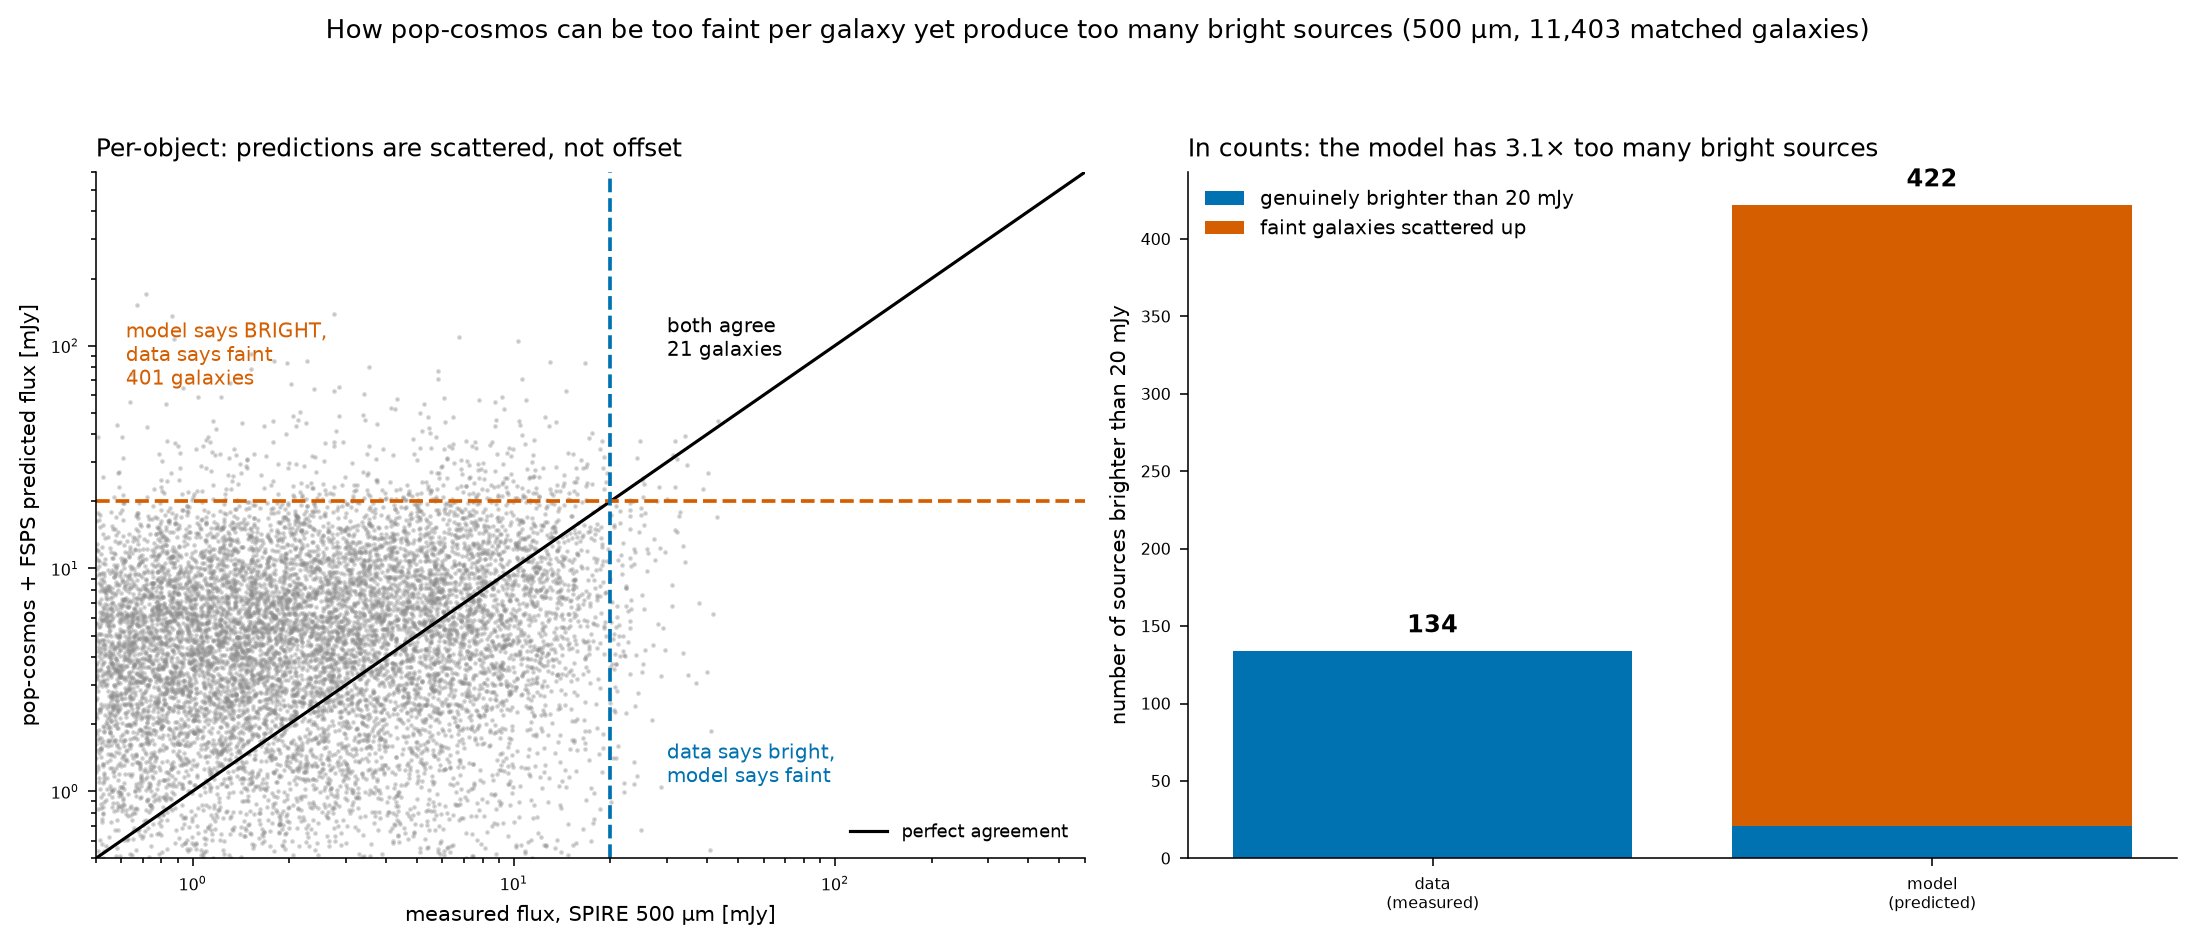
\includegraphics[width=1.15\textwidth]{Figures/scatter_mechanism_explained.png}}
\caption{Left: predicted vs observed \SI{500}{\um} flux for 11,403 finite matched galaxies,
showing the large per-object scatter. Right: 422 model galaxies are predicted above
\SI{20}{mJy}, while 134 are observed above the same threshold. Only 21 satisfy both
conditions. The remaining 401 model-bright galaxies are observed below the cut. In a
steeply falling source distribution, this broad upward redistribution can inflate the
bright counts even when the median prediction is too faint.}
\label{fig:scatter}
\end{figure}

Matched against the Wang catalogue, model galaxies show noise-deconvolved per-object
scatter of 0.45--\SI{0.52}{dex} (16--84th percentile half-width) at 250, 350 and
\SI{500}{\um}. The corresponding range against either Wang or Jin is
0.42--\SI{0.51}{dex}. This is far larger than the 0.12--\SI{0.15}{dex} agreement between the Wang and Jin
catalogues for the same sources. The scatter is therefore not explained by differences
between those deblending pipelines. It is stable under SNR cuts at 3, 5, 7 and
$10\sigma$, so observational noise near the detection limit does not drive it.

At the primary $\mathrm{SNR}\geq5$ cut, the median residuals are $-0.202$, $-0.313$ and
$-0.271$ dex at 250, 350 and \SI{500}{\um}. Thus the typical matched detection is too
faint in the model even though the full model catalogue produces too many bright
sources. Both statements are true simultaneously. Figure~\ref{fig:scatter} first
illustrates the threshold effect using all 11,403 finite
500~$\upmu$m matches. Of these, 422 model galaxies are predicted above \SI{20}{mJy},
but only 21 are also observed above that cut. By comparison, 134 matched galaxies are
observed above the cut. The broad model-to-observation residual distribution therefore
places many more galaxies in the model-bright sample than are supported by the observed
fluxes.

The numerical decomposition uses the wider $\mathrm{SNR}\geq3$ sample to retain enough
objects in every band. Table~\ref{tab:paradox} separates the count residuals into
contributions from the mean offset and from the scatter. At 250~$\upmu$m the scatter effect
($+\SI{0.55}{dex}$) fully accounts for the measured excess ($+\SI{0.19}{dex}$), with
the mean offset partially cancelling it. At 350 and 500~$\upmu$m the simple combination
of scatter and median offset predicts smaller excesses than are measured, leaving
residuals of $+0.20$ and $+0.15$ dex, respectively. This remaining term is consistent
with an additional population-level SED or count-shape mismatch, but the decomposition
does not identify a unique cause.

\begin{table}[H]
\centering
\caption{Decomposition of the count excess on the $\mathrm{SNR}\geq3$ matched sample
into contributions from the per-object mean offset and from scatter, at each SPIRE
wavelength.}
\label{tab:paradox}
\footnotesize
\begin{tabular}{@{}rrrrrr@{}}
\toprule
Band & Mean offset & Count effect & Scatter effect & Predicted net & Measured net \\
($\upmu$m) & (dex) & of mean (dex) & (dex) & (dex) & (dex) \\
\midrule
250 & $-0.163$ & $-0.361$ & $+0.549$ & $+0.19$ & $+0.19$ \\
350 & $-0.235$ & $-0.621$ & $+0.731$ & $+0.11$ & $+0.31$ \\
500 & $-0.183$ & $-0.575$ & $+0.855$ & $+0.28$ & $+0.43$ \\
\bottomrule
\end{tabular}
\end{table}

A warmer mean template can move the counts, but it does not by itself remove the
object-to-object scatter. These are two separate issues.

\subsection{Where the excess occurs in redshift}
\label{sec:results:redshift}

% FIGURE: z-resolved diagnosis
\begin{figure}[H]
\centering
\makebox[\textwidth][c]{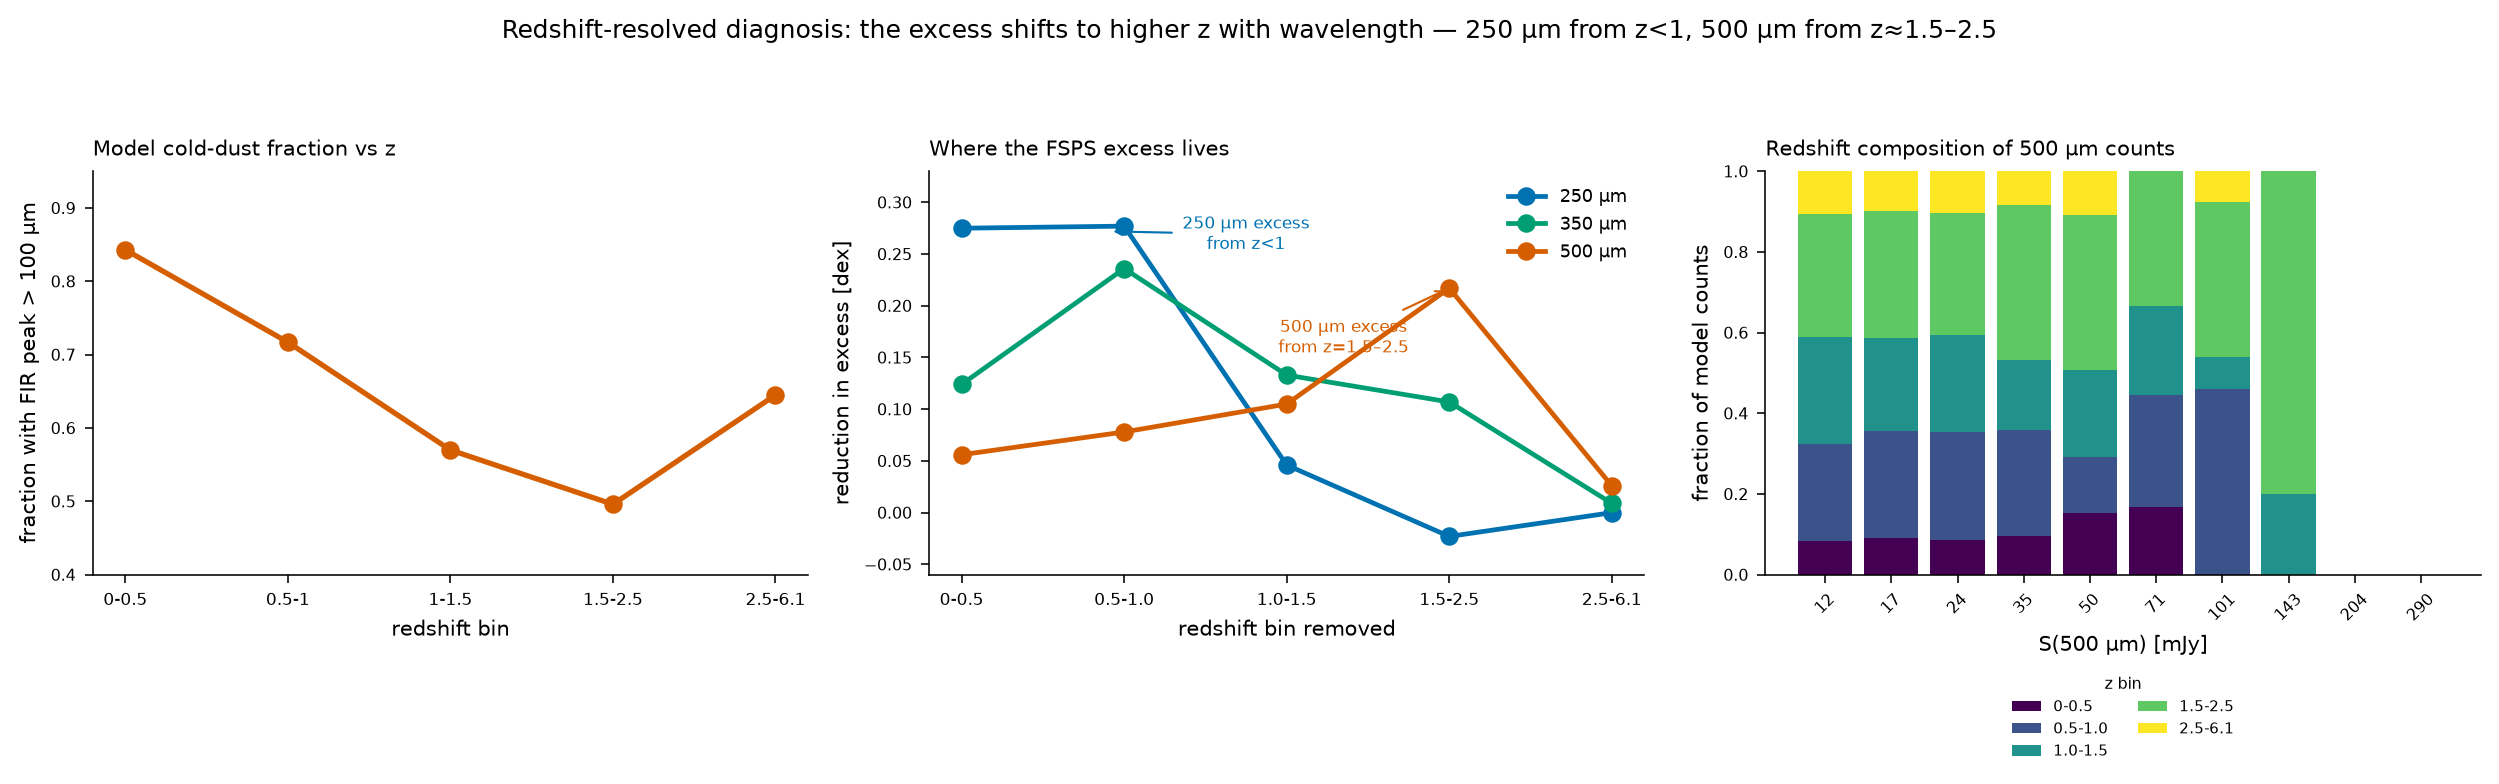
\includegraphics[width=1.15\textwidth]{Figures/z_resolved_fir_diagnosis.png}}
\caption{Change in median count residual when each redshift bin is excluded from the
model prediction. Larger improvement (taller bar) means that redshift bin contributes
more to the excess. At 250~$\upmu$m the excess is concentrated at $z < 1$; at
500~$\upmu$m it shifts to $z \approx 1.5$--$2.5$.}
\label{fig:z_resolved}
\end{figure}

The excess does not come from one universal redshift range. At 250~$\upmu$m, the
largest improvements come from excluding either $z<0.5$ or $0.5<z<1.0$, each reducing
the median residual by approximately \SI{0.28}{dex}. At 350~$\upmu$m the strongest
single contribution is $0.5<z<1.0$, with a \SI{0.24}{dex} improvement. At
500~$\upmu$m the excess shifts to $z \approx 1.5$--$2.5$, where exclusion improves the
residual by \SI{0.22}{dex}. Removing galaxies at $z>2.5$ changes the residual by less
than \SI{0.03}{dex} in every band. This band-dependent localisation is expected, because
the same observed wavelength samples different rest-frame wavelengths as redshift
changes. \citet{B_thermin_2012} found that the characteristic
contribution to SPIRE counts shifts to higher redshift at longer wavelengths, which is
consistent with this pattern. A direct numerical comparison against their
redshift-sliced counts was not performed and remains a useful extension.

This removal test is diagnostic rather than causal. Redshift is correlated with
luminosity, source abundance and the rest-frame wavelength sampled by a fixed observed
band. Removing a redshift interval changes all three together. The result therefore
locates the catalogue population responsible for the excess, but it does not on its own
show that redshift evolution is the missing model parameter.

\subsection{Observational side result: the Valiante bright-end uptick}
\label{sec:results:valiante}

While checking the observational inputs, an unexpected feature was found in the
\citet{Valiante_2016} H-ATLAS counts. In the brightest bins (above approximately
\SI{200}{mJy}), the Euclidean-normalised counts rise rather than continuing to fall.
The final \SI{300}{mJy} bin exceeds the \SI{244}{mJy} bin by approximately
$2.75\times$, $2.53\times$ and $2.17\times$ at 250, 350 and 500~$\upmu$m respectively.
The rise is present directly in the published tables and is not introduced by the
evaluator or a unit conversion.

Figure~\ref{fig:valiante_lensing} checks both the feature and a possible wavelength
dependence. Although the central uptick ratio decreases from 250 to 500~$\upmu$m, the
difference is less than $1\sigma$ after propagating the quoted errors. The data therefore
do not establish either a decrease or an increase with wavelength. The ratio errors are
only approximate because \citet{Valiante_2016} state that their quoted uncertainties do
not include correlations between flux bins.

% FIGURE: Valiante bright-end and lensing check
\begin{figure}[H]
\centering
\makebox[\textwidth][c]{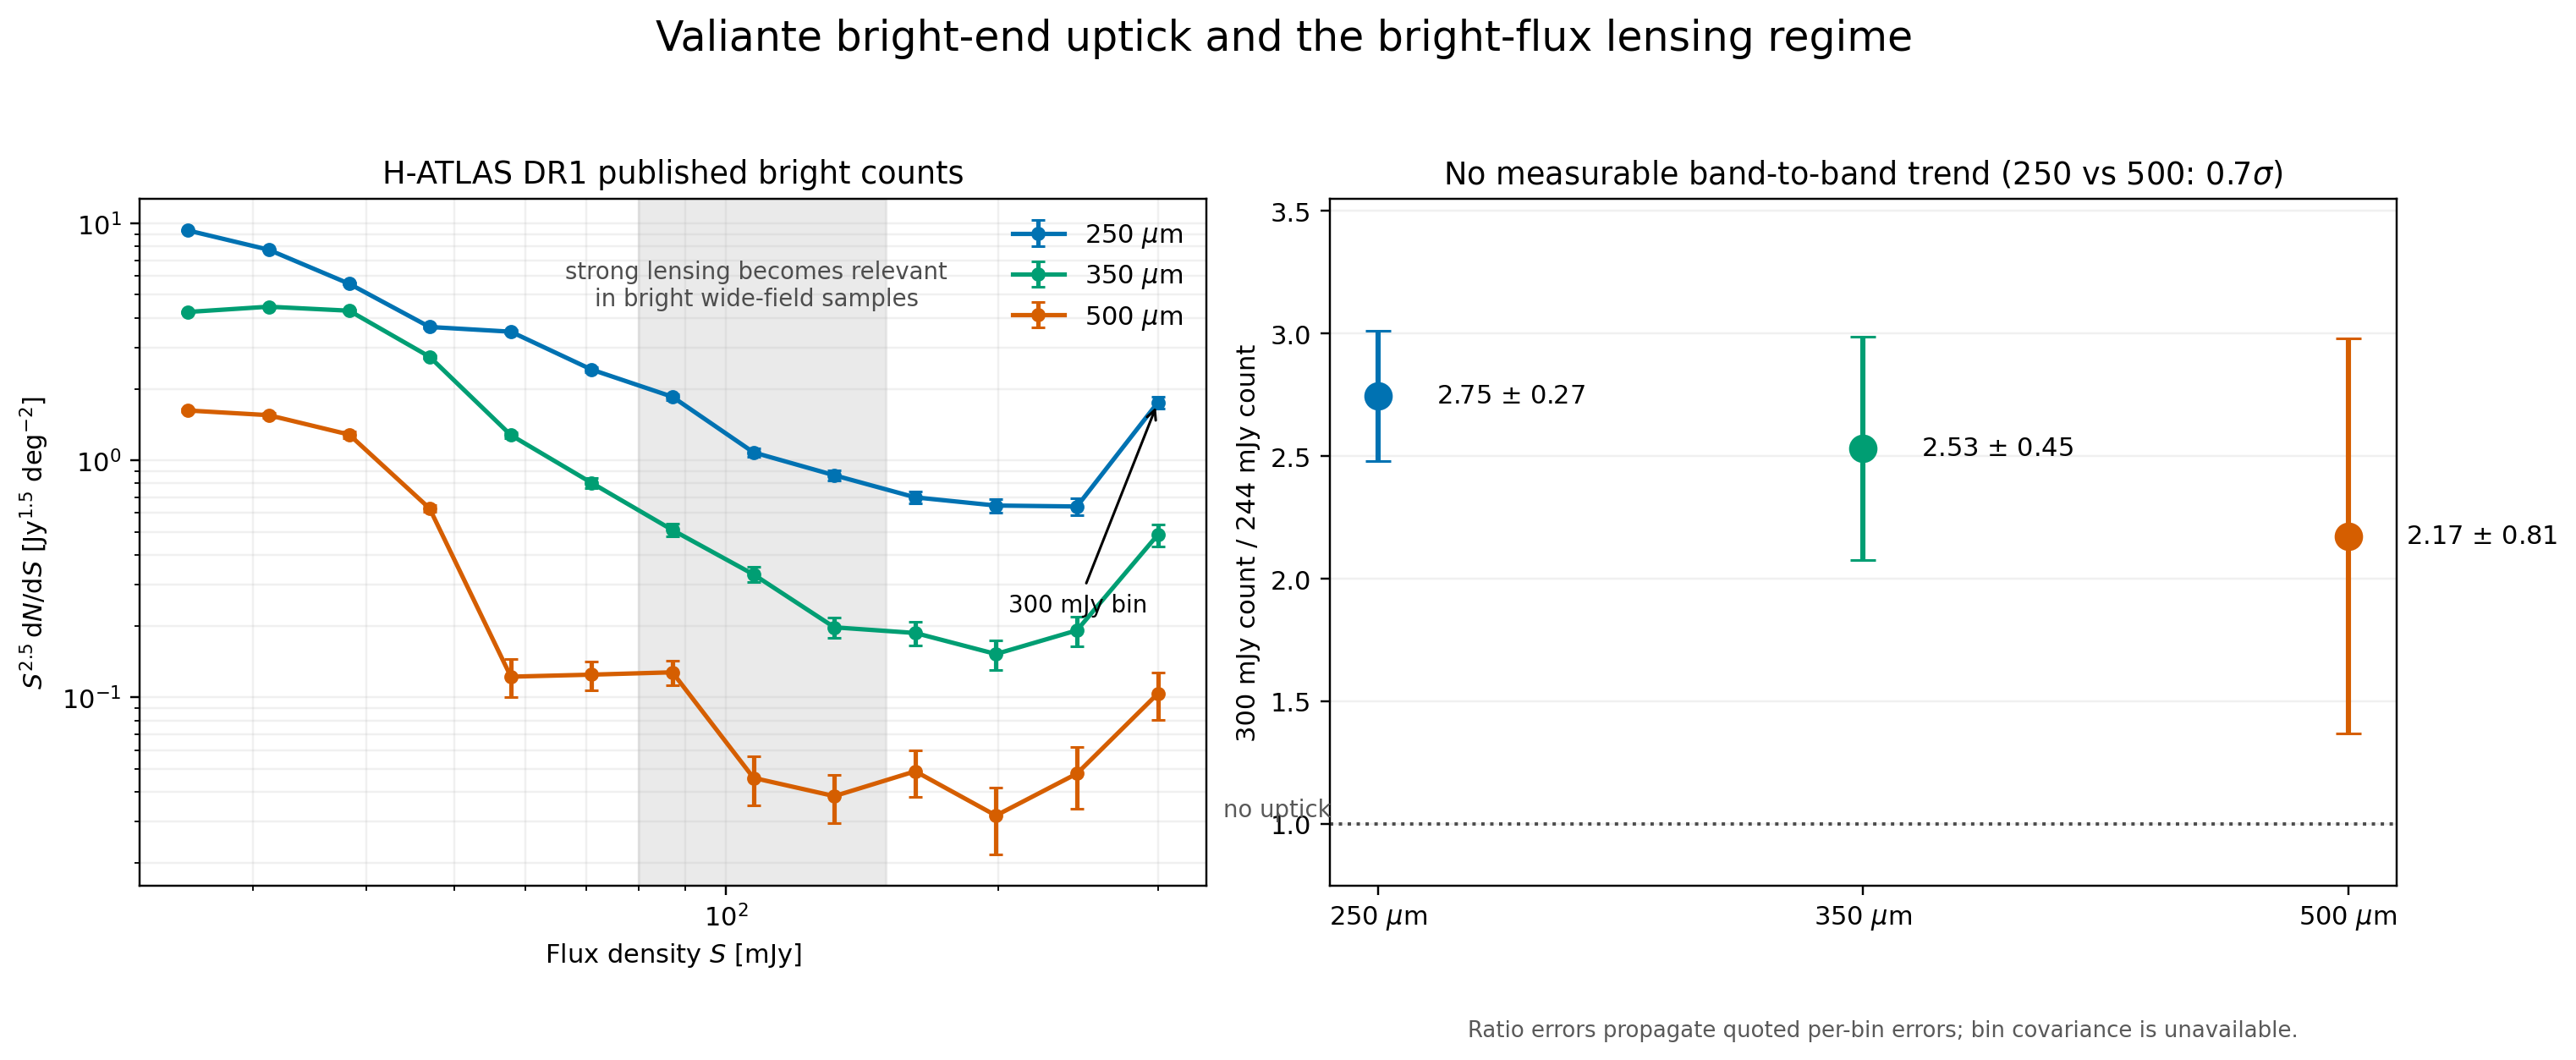
\includegraphics[width=1.15\textwidth]{Figures/lensing_bright_end_assessment.png}}
\caption{Left: area-weighted H-ATLAS DR1 counts transcribed from Tables 5, 8 and 9 of
\citet{Valiante_2016}. The shaded region marks the bright-flux range in which strong
lensing becomes relevant in wide-field submillimetre samples
\citep{Wardlow_2013,Negrello_2017}. It is contextual rather than a fit to the
Valiante data. Right: the \SI{300}{mJy} count divided by the \SI{244}{mJy} count in
each band. The central ratios decline with wavelength, but the differences are smaller
than the propagated uncertainties, so no wavelength trend is detected. The plotted
errors use the published per-bin uncertainties and omit unknown bin covariance.}
\label{fig:valiante_lensing}
\end{figure}

Lensing also cannot remove the \popcosmos{} bright-count excess. The published counts
already include magnified sources, whereas the model prediction contains no explicit
magnification step. If an illustrative 20\% lensed contribution is removed from the observed
100--\SI{300}{mJy} counts, the median model-minus-observation residual increases from
$+0.494$ to $+0.591$ dex at 250~$\upmu$m, from $+0.807$ to $+0.904$ dex at
350~$\upmu$m, and from $+1.165$ to $+1.262$ dex at 500~$\upmu$m. Thus lensing is an
important bright-end complication, but it acts in the wrong direction to explain why
the model is already above the observations.

\subsection{Robustness and alternative explanations}
\label{sec:results:robustness}

Five potential concerns were tested.

\textbf{Could one count survey drive the result?} The block bootstrap over independent
survey families keeps the FSPS offset positive (median $+\SI{0.29}{dex}$; 95\%
bootstrap interval $[+0.16,+0.52]$). This is treated as a robustness interval rather
than a formal confidence statement. The clean three-family evaluator
(Valiante, Oliver, Pearson) gives similar rankings to the full nine-source compilation.
Removing any single survey family does not change the sign of the excess.

\textbf{Could the Wang deblending be responsible for the scatter?} Wang and Jin agree
with each other to 0.12--\SI{0.15}{dex}, while \popcosmos{} scatters by
0.42--\SI{0.51}{dex} against either catalogue. The Wang--Jin difference accounts for
7\% of the variance at 250~$\upmu$m and 13\% at 500~$\upmu$m. Most of the measured
variance is therefore not represented by the difference between these catalogues.

\textbf{Could SNR selection explain it?} The per-object scatter is stable under SNR
cuts of 3, 5, 7 and $10\sigma$. At 250~$\upmu$m the noise-deconvolved scatter is
0.508, 0.515, 0.529 and \SI{0.539}{dex}, respectively. Across the same cuts it remains
within 0.441--\SI{0.499}{dex} at 350 and 500~$\upmu$m. The median offset becomes more
negative as the cut becomes stricter, but the scatter does not decrease. If noise near
the detection limit caused the broad distribution, the scatter should decrease.

\textbf{Could AGN dominate the cold-dust result?} The Drew--Casey peak-relation
comparison uses a low-AGN sample ($f_\mathrm{AGN} < 0.1$), which excludes the
hot-peaking branch. The cold, flat-slope result is still seen in this clean sample. The AGN
posterior-median limitation is discussed in
Section~\ref{sec:discussion:strength}.

\textbf{Could lensing dominate?} The central count claim is restricted to
10--\SI{100}{mJy}. Brighter bins are shown but do not support the headline numerical claim.
Strong lensing becomes increasingly important at the bright 500~$\upmu$m end, but the
sensitivity test in Section~\ref{sec:results:valiante} shows that removing an illustrative
lensed contribution from the observations makes the model excess larger rather than smaller.

\section{Discussion}
\label{sec:discussion}

\subsection{What the validation says about \popcosmos{}}
\label{sec:discussion:summary}

The optical and near-infrared control shows that the catalogue and flux pipeline work
well over the wavelengths used to constrain \popcosmos{}. The far-infrared tests reveal
two different limitations in the extrapolation.

The first is a population-level SED-shape problem. The baseline dust emission peaks near
\SI{136}{\um} in the rest frame and changes little with luminosity. At fixed \LIR{}, this
cold shape places more emission at long wavelengths and produces too many sources in the
SPIRE count bins. Warmer substitutions improve the counts, showing that far-infrared SED
shape is an important lever. The tests do not establish that the stored \LIR{} values are
physically correct or identify a unique replacement dust model.

The second limitation is object-level scatter. Individual predicted fluxes scatter by
0.42--\SI{0.51}{dex} against Wang and Jin. Replacing only the mean far-infrared template
can move the population counts but does not remove this broad galaxy-to-galaxy mismatch.
The two findings therefore require related but distinct improvements.

\subsection{Physical interpretation of the cold and uniform FIR shape}
\label{sec:discussion:cold}

Energy balance fixes the integral of dust emission from 8 to \SI{1000}{\um}, but it does
not determine how that energy is distributed over wavelength. The present analysis does
not independently validate or reject \LIR{}. It shows that the restricted dust-shape
assumptions used in this \popcosmos{} configuration are inadequate for reliable
far-infrared prediction.

The comparison with \citet{Drew_2022} gives this result a physical interpretation.
Observed galaxies follow a relation in which more luminous systems have warmer dust and
shorter peak wavelengths. Within the same $z\leq2$ calibration range, low-AGN
\popcosmos{} galaxies have a nearly flat relation and a fitted peak approximately
\SI{34}{\um} longer than the observed relation at
$L_\mathrm{IR}=10^{12}\,L_\odot$. The missing luminosity--temperature dependence offers
a plausible explanation for the especially large count excess at 350 and
500~$\upmu$m, where a cold template can deliver substantial flux.

In the Draine and Li framework, this missing trend points to the distribution of
radiation-field intensities rather than to the total energy. Increasing
$U_{\min}$ for more luminous galaxies would heat the diffuse component and shift
the far-infrared peak to shorter wavelengths. Varying $\gamma$ would alter the
fraction of dust exposed to stronger radiation fields and add galaxy-to-galaxy variation
in the warm tail. Adjusting $q_{\mathrm{PAH}}$  mainly affects the mid-infrared PAH
features, and is unlikely to remove the 350 and 500~$\upmu$m count excess by itself.
Although the present results do not measure these parameters directly, they do identify which physical features a future \popcosmos{} extension should allow to vary.

The controlled template substitutions support the same conclusion from a different
direction. Modified blackbodies, ALESS hybrids and Casey-style models all move the
counts toward agreement when given a warmer shape at fixed \LIR{}
\citep{Casey_2012,daCunha_2015}. However, several template families score similarly
within the inter-survey scatter, so the counts identify a needed direction (warmer and
luminosity-dependent) but do not uniquely select a dust prescription. The best
chi-square score should not be interpreted as identifying the correct grain model.

The hypothesis supported by this work is that \popcosmos{} needs a galaxy-dependent
far-infrared shape, likely linked to \LIR{} and potentially to redshift, compactness
or radiation-field intensity, rather than one effectively frozen cold-dust shape.

The hot SED branch does not weaken this cold-dust conclusion because the two populations
were separated before fitting the peak relation. It does, however, have an important
methodological implication. A median stacked SED remains cold even when a substantial
fraction of its constituent galaxies have short-wavelength, AGN-associated peaks.
Population stacks should therefore
be accompanied by distributions of individual SED properties. The association
between the hot branch and $f_\mathrm{AGN}$ is physically plausible, but its frequency
cannot yet be interpreted as a measured AGN fraction. The fitted parameter has a
bimodal prior and only posterior medians were available for the generated SEDs. Full
posteriors are needed to properly distinguish constrained AGN emission from
prior-driven branch selection.

\subsection{Why the number counts and individual fluxes appear to disagree}
\label{sec:discussion:paradox}

Published counts say the model produces too many bright objects. Matched Wang and Jin
galaxies say the model is typically too faint. Both can be true because of the shape of
the source distribution.

The per-object scatter of approximately \SI{0.45}{dex} moves galaxies both upward and
downward in flux. But because faint galaxies greatly outnumber bright ones, far more
objects scatter upward across a bright threshold than scatter downward across it. This
uneven promotion inflates the bright counts even as the median matched galaxy is
underpredicted. At 250~$\upmu$m the scatter effect accounts for the full measured
excess in the simple decomposition. At 350 and 500~$\upmu$m the combination of the
measured scatter and median offset leaves a smaller residual. That residual is consistent
with a further population-level mismatch, but this calculation does not assign it to one
physical cause.

The Wang--Jin agreement provides a useful control. The two deblending catalogues agree with
each other to 0.12--\SI{0.15}{dex}, far better than either agrees with \popcosmos{}
at 0.42--\SI{0.51}{dex}. One deblending routine is therefore unlikely to explain the
scatter. Wang and Jin do share the COSMOS field and related prior information, so their
agreement is a cross-check rather than a fully independent validation.

This implies that population summaries and per-object residuals test different
properties of the model. Matching counts alone could hide poor individual predictions,
while matching the median object alone could hide count inflation. Future validation
should therefore report both.

\subsection{How strong are the conclusions?}
\label{sec:discussion:strength}

Several conclusions are robust within the limits of the assembled data. The sign of the baseline count excess is stable across
all three independent survey families. The excess grows toward longer SPIRE wavelengths.
Warmer template shapes improve the agreement. Large per-object scatter appears against
both Wang and Jin. These findings remain under changes to the error floor, source selection and
the bootstrap resampling.

Other conclusions remain tentative. The exact preferred temperature or template family
depends on the error floor and flux range. Formal interpretation of the chi-square scores
is limited by correlated bins within each survey. The AGN analysis relies on posterior
medians of a parameter with a bimodal prior
\citep{Thorp_2025_insights}. Conclusions drawn above \SI{100}{mJy} are weak due to the
small COSMOS area, cosmic variance and the increased contribution of gravitationally
lensed sources.

The main limitations and their effects are as follows. Only three independent survey
families are available, with correlated bins inside each, so the error floor and block
bootstrap test robustness rather than provide a full likelihood. The COSMOS area of
\SI{1.278}{\deg\squared} gives few very bright sources. Nominal SPIRE wavelengths were
sampled rather than obtained by integrating through full filter transmission curves. SEDs use
posterior-median parameters rather than full posterior propagation, which may hide
bimodality in $f_\mathrm{AGN}$ and other parameters. The ALESS template represents
luminous submillimetre galaxies and is not a universal model
  \citep{daCunha_2015}. None of the experiments retrain the population prior jointly
  with far-infrared data. They replace the far-infrared extension after
inference. These limitations weaken the selection of a particular replacement model more
than the central result that the baseline far-infrared treatment needs improvement. The
most reliable count comparison is approximately 10--\SI{100}{mJy}.

\subsection{The Valiante bright-end uptick}
\label{sec:discussion:valiante}

The uptick in the brightest Valiante bins (Section~\ref{sec:results:valiante}) appears
in the area-weighted result in all three bands, so it is not introduced by the evaluator
or unit conversion. At the field level, all three GAMA fields rise at 250 and
350~$\upmu$m. At 500~$\upmu$m, GAMA12 and GAMA15 rise while GAMA9 falls, showing how
unstable the sparsest bright bins are. \citet{Valiante_2016} report that the GAMA fields
differ most at their brightest flux densities and attribute this to cosmic variance.
Rare nearby galaxies, small-number statistics, gravitational lensing and the
count-inversion procedure may also contribute, but this work cannot separate them.

Strong lensing is particularly relevant to very bright 500~$\upmu$m-selected samples
\citep{Wardlow_2013,Negrello_2017}. However, the Valiante band ratios do not show a
statistically measurable trend toward a stronger 500~$\upmu$m uptick. This does not rule
out a lensing contribution. It means only that these sparse bins cannot identify one.
More importantly, lensing cannot remove the model's bright-count excess. The published
counts already include magnified sources. Adding an explicit magnification step to
\popcosmos{} without changing the underlying population would increase its predicted
bright counts and worsen the disagreement.

Lensing creates a separate problem for matched-object validation. In a
strongly lensed system the optical and near-infrared light can be dominated by the
foreground lens while the far-infrared light comes from the magnified background
galaxy. A model constrained by the former cannot predict the latter through a different
dust template. This effect is negligible for the current COSMOS statistic. At
$\mathrm{SNR}\geq5$, the Wang catalogue contains one object above \SI{100}{mJy} at
250~$\upmu$m and none at 350 or 500~$\upmu$m. It should nevertheless be treated
explicitly if validation is extended to a much wider field. The present result supports
caution above \SI{100}{mJy}, not a new population or a lensing-based correction to the
main discrepancy.


\subsection{Implications and recommended extension of \popcosmos{}}
\label{sec:discussion:recommendations}

The results suggest several priorities for future \popcosmos{} work.

The most direct physical extension is to replace the fixed far-infrared bump with a
galaxy-dependent physical dust-emission family. Variable Draine and Li parameters, such
as radiation-field intensity and warm-dust fraction \citep{Draine_2007}, or alternative
dust modules available through CIGALE \citep{Boquien_2019}, would allow the far-infrared shape to respond to
galaxy properties. The Casey and ALESS templates used here are useful directional diagnostics but are not
recommended as final endpoint models.

At the population level, a conditional relation between far-infrared shape and
properties such as \LIR{}, redshift and SFR should be introduced. It can initially be guided by
the observed $L_\mathrm{IR}$--$\lambda_\mathrm{peak}$ relation. This relation should
include scatter rather than assigning one fixed template to every galaxy at a
given luminosity.

Future claims would be stronger if calibration and validation used separate data. One
set of independent survey fields could constrain the dust extension, while held-out
fields test it. Differential counts should be scored by band and flux regime, with per-object bias
and scatter against the deblended catalogues. Redshift-sliced counts or stacking
constraints from \citet{B_thermin_2012} could be used to test whether a correction is being applied
to the right population.

Technical improvements include integration through the true SPIRE bandpasses,
propagating posterior samples for the high-AGN and extreme-SFR populations, and
modelling survey selection and covariance explicitly where possible.

This work extends \popcosmos{} validation beyond its constraining wavelengths, identifies
where the extrapolation fails, provides evidence for why it fails, and presents a reproducible
evaluation framework for testing the next physical dust prescription.

\section{Conclusions}
\label{sec:conclusions}

This project tested whether \popcosmos{}, a generative galaxy population model
constrained at optical and near-infrared wavelengths, can make reliable predictions in the
\emph{Herschel}/SPIRE bands at 250, 350 and \SI{500}{\um}. The validation used
published differential number counts and matched COSMOS catalogues as directly observed
benchmarks rather than relying on derived physical quantities. The model works well over
its constraining wavelengths, but its current far-infrared extension does not reliably
reproduce either population counts or individual galaxy fluxes.

Nine published count products from six papers were placed in common units and grouped
into three independent survey families, with overlapping products retained as checks.
The baseline \popcosmos{}/FSPS prediction overpredicts the counts in all three
bands. Over the 30--\SI{100}{mJy} range where all three families overlap, the excess is
approximately $1.7\times$ at 250 and 350~$\upmu$m and $3.6\times$ at 500~$\upmu$m. As a
control, IRAC Ch1 and Ch2 residuals are only a few hundredths of a magnitude, confirming
that the mismatch is wavelength-specific rather than a broken catalogue or flux pipeline.

The physical diagnosis is that the baseline far-infrared dust bump is too cold and too
uniform. At $L_\mathrm{IR} = 10^{12}\,L_\odot$, model galaxies peak near
\SI{126}{\um} rather than the observed \SI{92}{\um}. Over the observed calibration
range $z\leq2$, the model shows essentially no luminosity dependence
($\eta=+0.004$ compared with $-0.09$). Preserving each
galaxy's total \LIR{} while substituting warmer dust shapes (modified blackbodies,
ALESS/FSPS hybrids, Casey-style models) improves the counts. Their similar performance
identifies the required direction, warmer and luminosity-dependent, but does not
select a unique physical dust model. The full catalogue also contains a distinct hot,
AGN-associated SED branch near \SI{14}{\um}. Its presence is hidden by median stacks and
its population fraction remains uncertain because the analysis uses posterior-median
parameters rather than full posterior samples.

A separate limitation emerged from the per-object comparison. Model fluxes scatter by
0.42--\SI{0.51}{dex} against Wang or Jin, while those two catalogues agree with each
other to 0.12--\SI{0.15}{dex}. The median matched galaxy is underpredicted, yet
the model still overproduces bright counts, because the steep source distribution and
large scatter move many more faint objects upward than bright objects downward.
Changing the mean dust template improves the counts but does not remove this large
object-to-object scatter. Population bias and individual scatter must therefore both be
addressed.

The excess keeps the same sign across all three independent survey families under
changes to the error floor and source selection. The per-object scatter also persists
under SNR cuts from 3 to $10\sigma$. The block bootstrap gives a median baseline offset
of $+\SI{0.29}{dex}$ with an interval of $[+0.16,+0.52]$. This is a robustness
summary rather than a formal exclusion. The main limitations are correlated bins within
each survey, only three independent families, nominal-wavelength rather than
full-bandpass fluxes, posterior medians rather than full posterior propagation, and weak
bright-end statistics in a COSMOS-sized area. The Valiante bright-end uptick was
confirmed in the published tables, but its origin was not resolved. Results above
approximately \SI{100}{mJy} should therefore be interpreted cautiously.

The main recommendation for \popcosmos{} is to preserve the learned population model and
energy balance while adding a galaxy-dependent far-infrared dust
family linked to \LIR{} and potentially redshift and SFR, with intrinsic scatter.
Variable Draine and Li parameters \citep{Draine_2007} or alternative dust modules
available through CIGALE \citep{Boquien_2019} provide possible starting points. Future validation should calibrate
on one set of survey fields and test on held-out fields, reporting both differential
count performance and per-object flux scatter. More generally, a generative population
model can reproduce observables within its calibration range while failing at unseen
wavelengths. Validation beyond that range requires both population distributions and
individual-object tests.

\section*{Acknowledgements}
I would like to thank my supervisors, David Clements and Boris Leistedt, for their
guidance, feedback and encouragement throughout this project. I am particularly
grateful to Boris for providing the \popcosmos{} SED products and supporting data used
in the analysis, and to David for his advice and expertise on the far-infrared observations and the
interpretation of the results. I also thank the \popcosmos{} collaboration and the
teams behind the public COSMOS and \emph{Herschel} catalogues whose work made this
study possible.

% ===================== AI USE DECLARATION =====================
% Imperial requires this to be accurate and specific. EDIT to reflect exactly what
% you used and how. A vague declaration is worse than none.
\FloatBarrier
\section*{AI Use Declaration}
Generative AI tools were used in the preparation of this report in the following
ways. They assisted with code development and debugging, literature discovery,
cross-checking numerical summaries, planning the report structure, editing prose and
LaTeX formatting. The author reviewed the cited sources, analysis choices, numerical
results, scientific interpretation and final text, and takes responsibility for the
submitted report.

% ===================== BIBLIOGRAPHY =====================
\bibliographystyle{apalike}
\bibliography{references}

\end{document}
